% **************************************************************************************************************
%
%  Copyright 2020-2026 Robert Bosch GmbH
%
%  Licensed under the Apache License, Version 2.0 (the "License");
%  you may not use this file except in compliance with the License.
%  You may obtain a copy of the License at
%
%      http://www.apache.org/licenses/LICENSE-2.0
%
%  Unless required by applicable law or agreed to in writing, software
%  distributed under the License is distributed on an "AS IS" BASIS,
%  WITHOUT WARRANTIES OR CONDITIONS OF ANY KIND, either express or implied.
%  See the License for the specific language governing permissions and
%  limitations under the License.
%
% **************************************************************************************************************

\section{Description}

\subsection{Overview}

MicroserviceBase is a framework for building microservices in Python or C++ that talk
\textbf{gRPC over HTTP/2}, register themselves in a \textbf{HashiCorp Consul} service
catalog, and run as \textbf{HashiCorp Nomad} jobs.  A \textbf{FastAPI bridge} hosts the
REST endpoints used by the cross-platform \textbf{Manager GUI}, and the same endpoints
are usable from \texttt{curl} or any scripting language.  All generated code follows
\textbf{hexagonal architecture} (domain / ports / adapters), so the transport,
discovery, and orchestration choices stay confined to the adapter layer and never leak
into the business logic.

\begin{figure}[!htb]
\centering
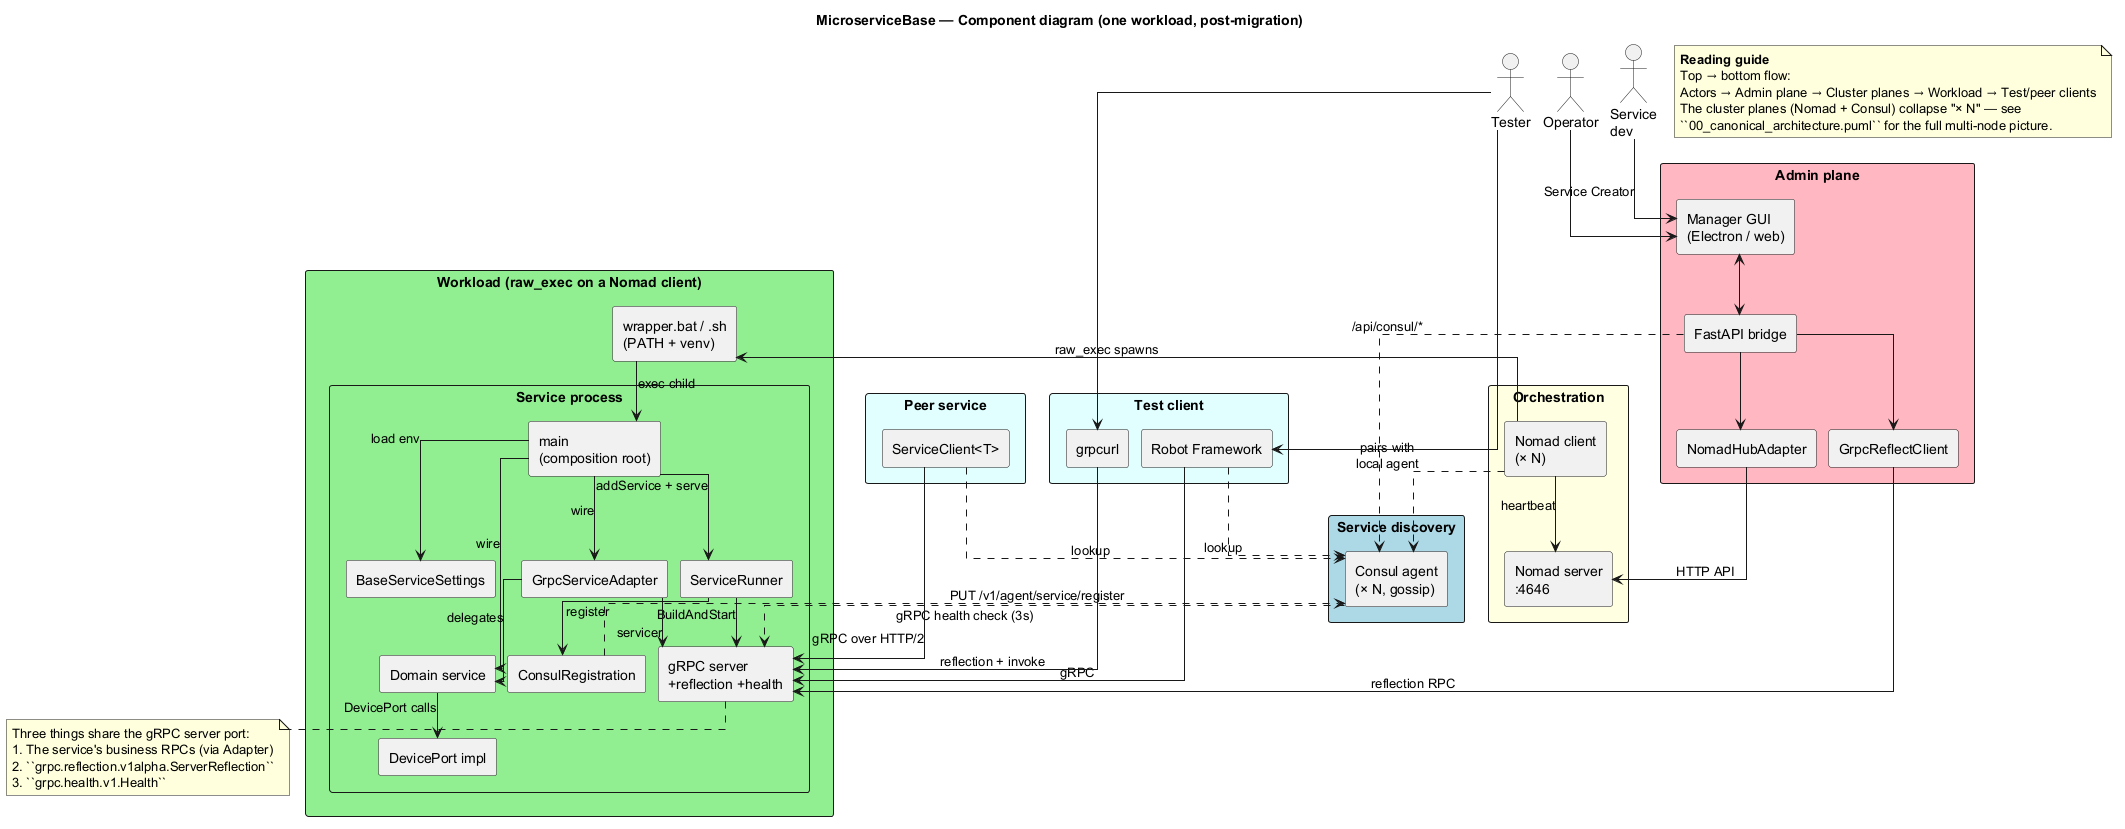
\includegraphics[width=0.95\textwidth]{pictures/overview.png}
\caption{MicroserviceBase System Overview}
\label{fig:overview}
\end{figure}

\subsubsection{Key Features}

\begin{itemize}
   \item \textbf{gRPC + reflection}: services advertise their methods and message
         schemas at runtime through the standard \texttt{grpc.reflection} plugin --
         clients enumerate without a local \texttt{.proto}
   \item \textbf{Consul service catalog}: every service self-registers on startup with
         name, dynamic port, health check, and a \texttt{grpc\_services} meta tag, and
         deregisters cleanly on shutdown
   \item \textbf{Nomad orchestration}: every generated project ships
         \texttt{deploy/<svc>.nomad.hcl} with a single \texttt{raw\_exec} task and a
         dynamic \texttt{grpc} port; the same job runs on Windows and Linux
   \item \textbf{Hexagonal scaffold for Python and C++}: \texttt{mb-scaffold} (CLI) and
         the \textbf{Service Creator wizard} (GUI) emit a complete project with
         \texttt{domain/}, \texttt{adapters/}, \texttt{proto/}, \texttt{deploy/}, build
         scripts, and an optional \texttt{GUIs/} plugin
   \item \textbf{C++ build via vcpkg}: a project-local
         \texttt{vcpkg-overlay-ports/grpc/} forces
         \texttt{gRPC\_BUILD\_GRPC\_CPP\_REFLECTION\_PLUGIN=ON} so reflection is always
         available regardless of the upstream port's defaults
   \item \textbf{FastAPI bridge}: \texttt{/api/scaffold}, \texttt{/api/grpc},
         \texttt{/api/consul}, \texttt{/api/nomad} -- one process, four namespaces;
         used by the GUI and equally by automation scripts
   \item \textbf{Manager GUI}: dual-host (Electron desktop + browser) with a
         Consul-driven Services sidebar, a Service Network tab for managing the agents,
         and a Service Creator wizard
   \item \textbf{QConnectBase \texttt{GrpcClient}}: contributed upstream so Robot
         Framework tests drive gRPC services with the same keyword model used for TCP,
         Serial, SSH, and the legacy RabbitMQ broker
   \item \textbf{Standalone installers}: NSIS for Windows (with Consul / Nomad detection
         + \texttt{winget} install fallbacks), \texttt{.deb} / AppImage for Linux (with
         a \texttt{bootstrap.sh} that installs the agents from the official HashiCorp
         repos)
\end{itemize}

\subsubsection{Design Philosophy}

\begin{enumerate}
   \item \textbf{Standards over bespoke}: gRPC, Consul, Nomad -- pick the boring,
         widely-used building blocks instead of inventing transport / discovery /
         orchestration in-house
   \item \textbf{Hexagonal architecture}: domain code never imports gRPC, Consul, Nomad,
         FastAPI, or Qt; swapping a transport is purely an adapter problem
   \item \textbf{Same code generates same shape}: \texttt{mb-scaffold} produces the same
         file layout for Python and C++, single-service and multi-proto, so a developer
         familiar with one knows the other on sight
   \item \textbf{Reflect-first, fall back to compile}: clients prefer gRPC reflection
         and only compile a local \texttt{.proto} (\texttt{LocalProtoClient}) when
         reflection is not available
   \item \textbf{Graceful shutdown on every platform}: Python services convert
         \texttt{SIGBREAK} (Windows) and \texttt{SIGTERM} (Linux) into a clean
         deregister-then-exit path; C++ services do the same via the \texttt{Server}
         shutdown handler
\end{enumerate}

% ============================================================================
\subsection{Architecture}
% ============================================================================

MicroserviceBase is organised into the classic hexagonal layers, applied uniformly to
both the framework itself and to every generated service:

\begin{figure}[!htb]
\centering
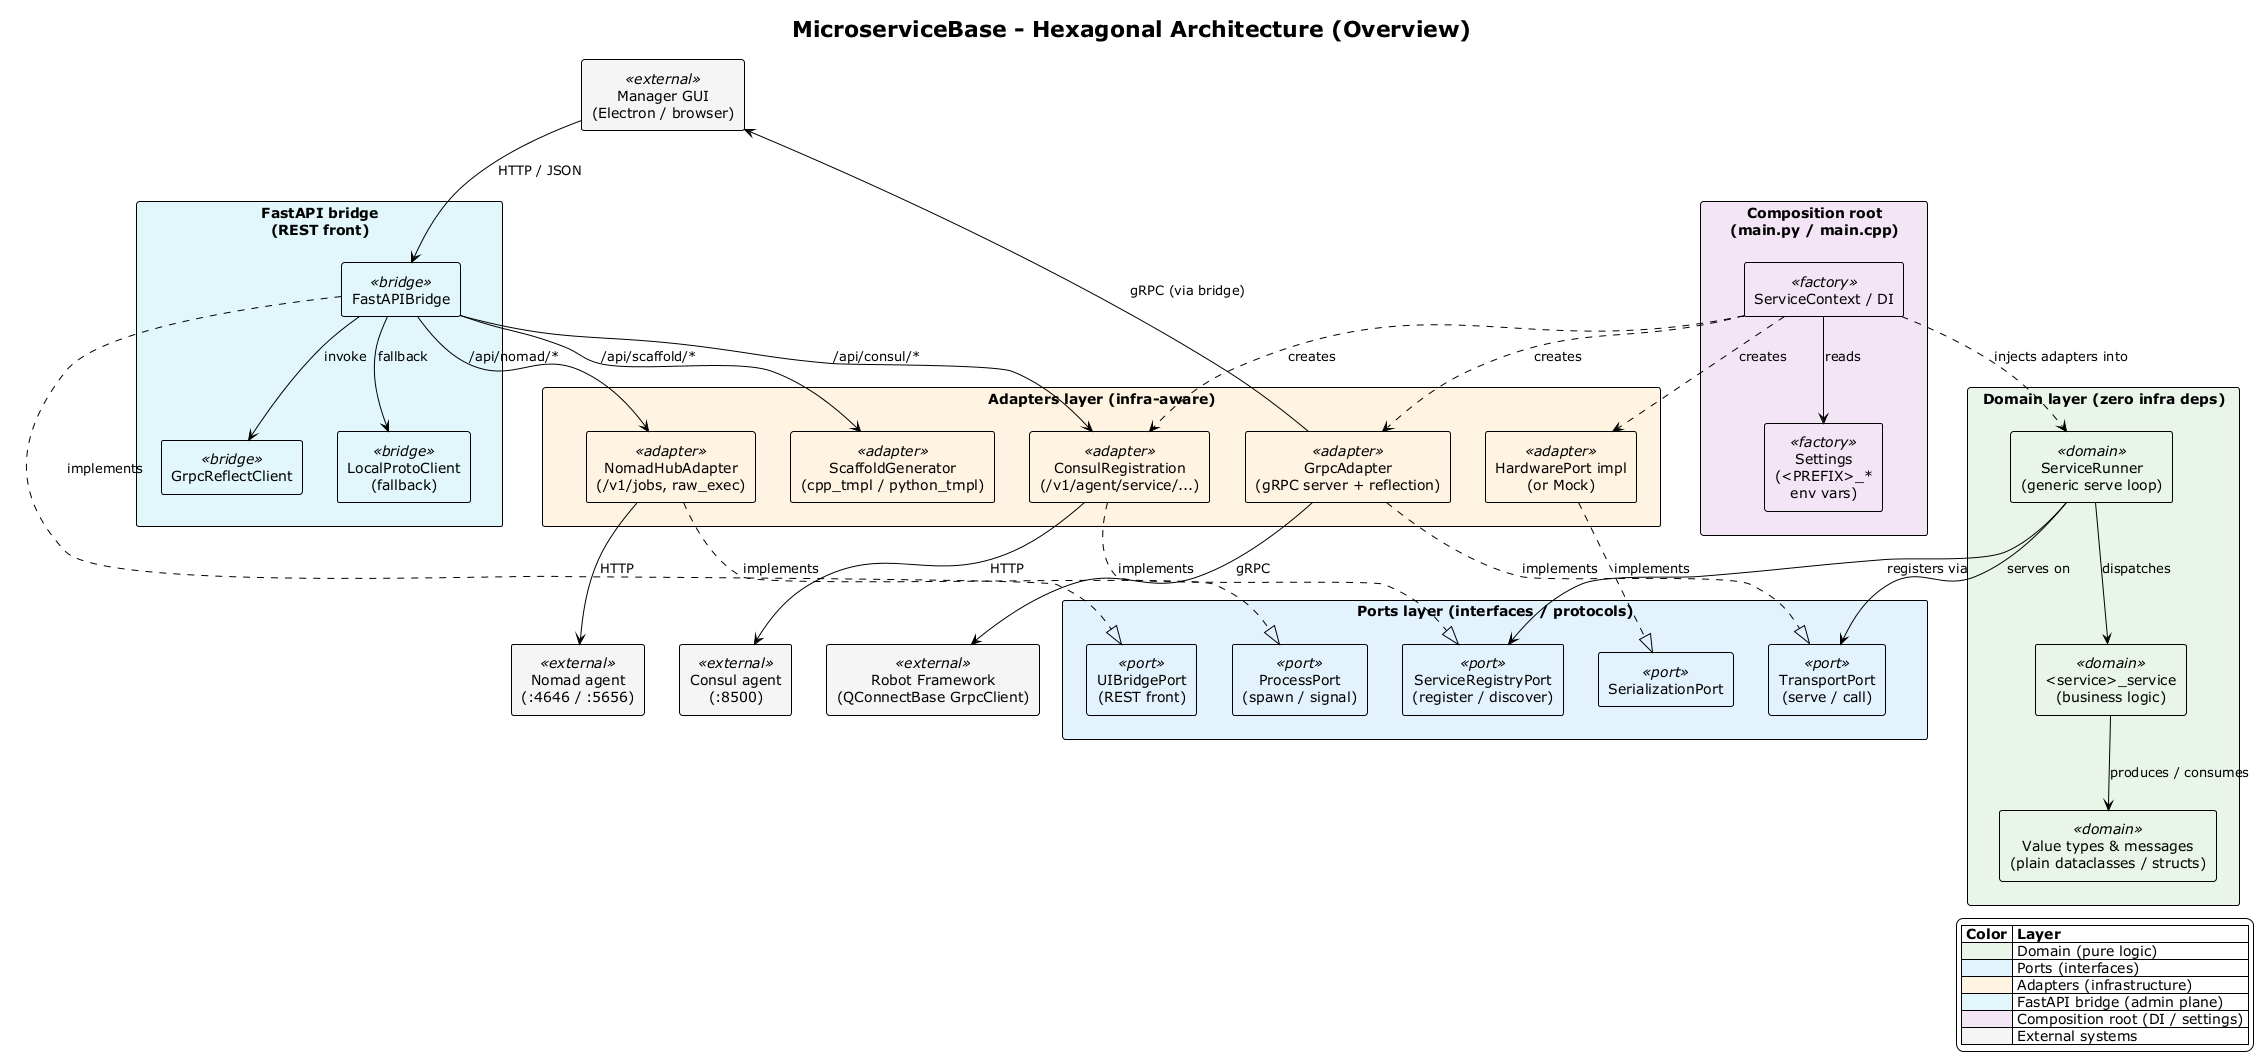
\includegraphics[width=0.95\textwidth]{pictures/architecture_overview.png}
\caption{Hexagonal Architecture Overview}
\label{fig:architecture_overview}
\end{figure}

\noindent
The detailed architecture with the major adapters (gRPC, Consul, Nomad, FastAPI bridge,
scaffold generator) wired through their port interfaces:

\begin{figure}[!htb]
\centering
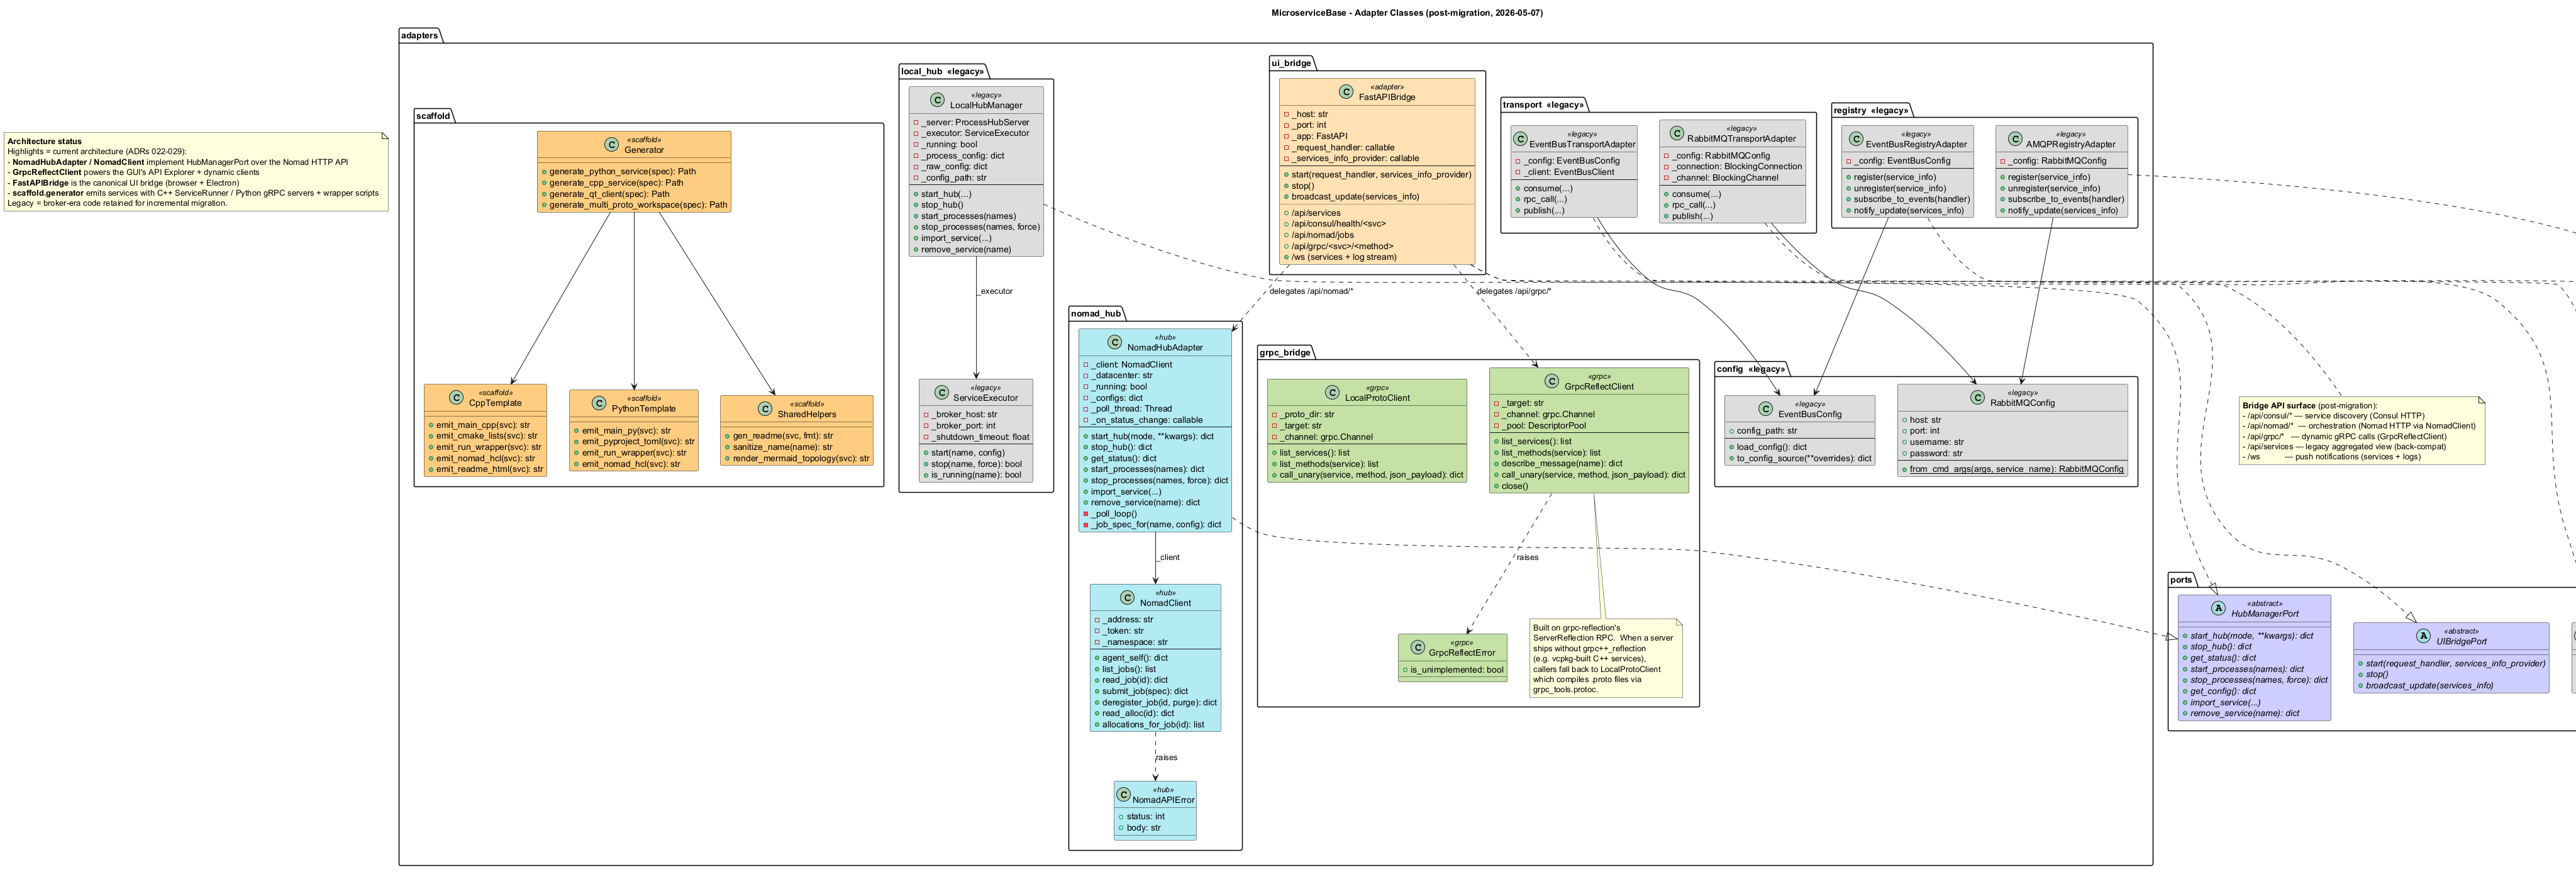
\includegraphics[width=0.95\textwidth]{pictures/architecture_detail.png}
\caption{Hexagonal Architecture Detail}
\label{fig:architecture_detail}
\end{figure}

\subsubsection{Layer Responsibilities}

\begin{description}
   \item[Domain Layer] Pure business logic with zero infrastructure dependencies:
        \texttt{ServiceBase} (the abstract microservice contract), value types,
        and generated service classes
        (\texttt{src/<svc>/domain/<svc>\_service.\{py,cpp\}}).  The domain never imports
        \texttt{grpc}, \texttt{python-consul}, \texttt{fastapi}, \texttt{httpx}, or Qt
        and is unit-testable in isolation.

   \item[Ports Layer] Abstract protocol interfaces that the domain talks to:
        \texttt{TransportPort} (RPC in / out), \texttt{RegistryPort} (registration +
        discovery), \texttt{ProcessPort} (subprocess management),
        \texttt{SerializationPort}, and \texttt{UIBridgePort} (HTTP for the GUI).

   \item[Adapters Layer] Concrete infrastructure-aware implementations:
        \begin{itemize}
           \item \texttt{gRPC adapter} -- \texttt{adapters/grpc\_bridge/} -- request
                 routing, reflection client (\texttt{ReflectClient}), and a
                 \texttt{LocalProtoClient} fallback that compiles \texttt{.proto} files
                 with \texttt{grpc\_tools.protoc}
           \item \texttt{Consul adapter} -- \texttt{adapters/consul/} -- HTTP wrapper
                 around \texttt{/v1/agent/service/register},
                 \texttt{/v1/health/service/<name>?passing=true}, and the catalog
                 endpoints
           \item \texttt{Nomad adapter} -- \texttt{adapters/nomad/} -- agent lifecycle
                 (start / stop / status), job submission, and per-task status streaming
           \item \texttt{FastAPI bridge} -- \texttt{adapters/ui\_bridge/fastapi\_bridge.py}
                 -- the single REST front for the GUI; mounts the GUI's static assets
                 in browser mode
           \item \texttt{scaffold generator} -- \texttt{adapters/scaffold/cpp\_tmpl.py}
                 and \texttt{python\_tmpl.py} -- one templated emitter per output file;
                 backs both the wizard and the CLI
        \end{itemize}

   \item[GUI Layer] \texttt{MicroserviceManagerGUI} runs in two modes:
        \begin{itemize}
           \item \texttt{Electron} -- desktop wrapper with \texttt{contextBridge} preload
           \item \texttt{Web} -- pure browser-compatible HTML / CSS / JS, served by the
                 FastAPI bridge under \texttt{http://localhost:1112}
           \item \texttt{Service Plugins} -- per-service HTML + JS dropped into
                 \texttt{web/services/} and loaded into the Manager GUI namespace
                 (\texttt{window.MicroserviceManager}, alias \texttt{MM})
        \end{itemize}
\end{description}

% ============================================================================
\subsection{Components}
% ============================================================================

\subsubsection{Service Discovery: Consul}

Every service registers itself in Consul on startup with:

\begin{itemize}
   \item \textbf{Name}: snake-case service name (e.g.\ \texttt{analog\_input\_service})
   \item \textbf{Address + port}: where its gRPC server is listening
        (Nomad-allocated, exposed as the \texttt{\$\{NOMAD\_PORT\_grpc\}} env var)
   \item \textbf{Health check}: a TCP probe to the gRPC port, polled every few seconds
   \item \textbf{Tags}: \texttt{v1} (or whatever the service version is)
   \item \textbf{Meta}: \texttt{grpc\_services} -- comma-separated list of fully-qualified
        gRPC service names the binary implements (lets the GUI skip a reflection
        round-trip when listing services to enumerate)
\end{itemize}

\noindent
Clients resolve via \texttt{GET /v1/health/service/<name>?passing=true} which returns
the healthy \texttt{address:port} pairs.  The Manager GUI uses this for its Services
sidebar; \texttt{ServiceClient} uses it for outbound gRPC calls.  Local-dev typically
runs \texttt{consul agent -dev} (single-node, in-memory); the Manager GUI's
\textbf{Service Network} \(\to\) \textbf{Consul} tab can launch and manage that for you.

\subsubsection{Orchestration: Nomad}

Each generated service ships a \texttt{deploy/<svc>.nomad.hcl} job that declares:

\begin{itemize}
   \item A single task running the service binary under \texttt{raw\_exec}
   \item A dynamic port labelled \texttt{grpc} -- Nomad picks a free port and exports it
        as the \texttt{\$\{NOMAD\_PORT\_grpc\}} env var
   \item Environment variables to point the binary at Consul (\texttt{CONSUL\_ADDR})
\end{itemize}

\noindent
Submit with \texttt{nomad job run deploy/<svc>.nomad.hcl}, or via the GUI's Nomad tab
\(\to\) \textbf{Submit Job} dialog.  \texttt{raw\_exec} runs the process directly (no
container) so the same job works on Windows and Linux without Docker / cgroups setup.
For production you can swap to \texttt{exec} (Linux container) or \texttt{docker}
without changing the framework -- only the \texttt{.hcl} template.

\subsubsection{Method Discovery: gRPC Server Reflection}

Servers built with our scaffold include \texttt{grpc++\_reflection} (the vcpkg
overlay-port forces it on; see \texttt{changelog.html}) and call
\texttt{grpc::reflection::InitProtoReflectionServerBuilderPlugin()} at startup.
Clients can then enumerate services, methods, and message schemas at runtime
without any \texttt{.proto} file.  Fallback: when reflection is not available
(older servers, custom builds), the bridge can compile local \texttt{.proto}
files via \texttt{grpc\_tools.protoc} and use the descriptors that way -- see
\texttt{LocalProtoClient} in
\texttt{MicroserviceBase/adapters/grpc\_bridge/reflect\_client.py}.

\begin{figure}[!htb]
\centering

\includegraphics[width=0.85\textwidth]{pictures/sequence_communication.png}
\caption{Method discovery + invocation: GUI -- bridge -- Consul -- Service}
\label{fig:sequence_communication}
\end{figure}

\subsubsection{The FastAPI Bridge}

The bridge is a single Python process that:

\begin{enumerate}
   \item Hosts the Manager GUI's static assets at \texttt{/} (when running in browser
         mode, default \texttt{http://localhost:1112})
   \item Exposes REST endpoints for everything the GUI does:
         \begin{itemize}
            \item \texttt{/api/scaffold/...} -- generate service projects
                  (\texttt{mb-scaffold} backend)
            \item \texttt{/api/grpc/...} -- list methods + invoke (via reflect\_client)
            \item \texttt{/api/consul/...} -- start / stop the agent + read the catalog
            \item \texttt{/api/nomad/...} -- start / stop the agent + submit / stop jobs
         \end{itemize}
   \item Manages Consul + Nomad agents as Python subprocesses (PID-tracked in
         \texttt{\%TEMP\%/msbase\_*\_agent.pid} for restart resilience)
\end{enumerate}

\noindent
The GUI is a thin client over this -- every button maps to one or two endpoints.  The
same endpoints are usable from \texttt{curl} or scripts when automating.  Source:
\texttt{MicroserviceBase/adapters/ui\_bridge/fastapi\_bridge.py}.

\subsubsection{The Scaffold Generator}

\texttt{mb-scaffold} (\texttt{python -m MicroserviceBase.tools.scaffold\_cli}) emits a
complete service project from a small spec.  Three layout selectors are supported:

\begin{description}
   \item[\texttt{monorepo}] (default) -- N services share one \texttt{.proto}; each
        service compiles into its own binary
   \item[\texttt{multi\_proto}] -- N services from N separate \texttt{.proto} files,
        all hosted in one binary on one port with one Consul registration
   \item[\texttt{separate}] -- one service per project (degenerate case of monorepo)
\end{description}

\noindent
For Python the scaffold emits \texttt{main.py}, \texttt{config.py}, \texttt{context.py},
\texttt{pyproject.toml}, the hexagonal \texttt{domain/} and \texttt{adapters/api/}
folders, the \texttt{proto/} contract plus \texttt{scripts/generate\_protos.py}, and
optional \texttt{deploy/} (Nomad job + \texttt{*\_service\_config.json} for Consul) and
\texttt{GUIs/} (HTML + JS plugin) directories.  For C++ it additionally emits
\texttt{CMakeLists.txt}, \texttt{vcpkg.json}, the \texttt{vcpkg-overlay-ports/grpc/}
folder, and \texttt{build\_msvc.bat} / \texttt{build\_msys2.bat} wrappers.  Source:
\texttt{MicroserviceBase/adapters/scaffold/} (cpp\_tmpl.py + python\_tmpl.py).

\subsubsection{Generated Service Layout}

The same shape is produced for every service.  Files marked \emph{generic} are
templated and safe to regenerate; files marked \emph{specific} hold the parts you
actually write (your \texttt{.proto} contract and the corresponding domain class):

\begin{verbatim}
out/<service>/
+-- main.py | main.cpp           # Entry point (generic)
+-- config.py | config.h         # Settings, env vars, ports        (generic)
+-- context.py                   # ServiceContext / DI              (generic, Python)
+-- pyproject.toml               # uv / pip deps                    (generic, Python)
+-- CMakeLists.txt | vcpkg.json  # Build files                      (generic, C++)
+-- vcpkg-overlay-ports/grpc/    # Forces reflection plugin ON      (generic, C++)
+-- proto/<svc>.proto            # gRPC contract                    (SPECIFIC)
+-- domain/<svc>_service.{py,cpp}  # Business logic                 (SPECIFIC)
+-- adapters/api/grpc_adapter.{py,cpp}  # Servicer (proto -> domain) (generic)
+-- scripts/generate_protos.py   # Pre-builds *_pb2[_grpc].py       (generic, Python)
+-- deploy/<svc>.nomad.hcl       # Nomad raw_exec job               (generic)
+-- deploy/<svc>_service_config.json  # Consul registration meta    (generic)
+-- GUIs/<svc>.html | <svc>.js   # Optional Manager GUI plugin      (generic + custom)
+-- README.md                    # Build / run / deploy steps       (generic)
\end{verbatim}

\noindent
Re-running \texttt{mb-scaffold} on an existing project overwrites the generic files and
leaves the specific ones alone, so your \texttt{.proto} and domain code survive a
regen.

% ============================================================================
\subsection{Communication Patterns}
% ============================================================================

\subsubsection{RPC via gRPC over HTTP/2}

Clients call services through generated stubs (when they have the \texttt{.proto}) or
via the bridge's reflection-driven generic invoker (when they do not).  Below is the
generic-invoker path in Python -- the same call from JavaScript or Robot Framework goes
through the bridge in exactly the same way:

\begin{verbatim}
import httpx

# Resolve via Consul (handled by the bridge)
r = httpx.post("http://localhost:1112/api/grpc/invoke", json={
    "service": "calculator_service",            # Consul service name
    "method":  "Calculator.Add",                # FQN: <package>.<svc>.<method>
    "request": {"a": 1, "b": 2},                # message as JSON
})
print(r.json())   # {"result": 3}
\end{verbatim}

\noindent
The bridge looks the service up in Consul, opens a gRPC channel, calls the method
(synthesising stubs from reflection if required), and returns the response as JSON.
Stub-based calls for performance-critical paths are documented in the per-language
\texttt{README} that ships with every generated project.

\subsubsection{Service Registration}

Registration is automatic.  In Python, \texttt{ServiceBase.register\_service()} is
called from the generated \texttt{main.py} after the gRPC server has bound to its port;
in C++, the equivalent call lives in \texttt{main.cpp} after \texttt{Server::BuildAndStart()}.
Both speak directly to the local Consul agent over HTTP.  On clean shutdown the
service deregisters itself; if the process dies abruptly, Consul's TCP health check
fails it out of the catalog within a few seconds.

\subsubsection{Robot Framework: \texttt{GrpcClient}}

The QConnectBase \texttt{GrpcClient} connection type ships with this release
(\texttt{QConnectBase/grpc/grpc\_client.py}).  Robot tests drive gRPC services with the
same \texttt{Connect} / \texttt{Send Command} / \texttt{Verify} / \texttt{Disconnect}
keywords already in use for TCP, Serial, SSH, and the legacy RabbitMQ broker -- and
support both modes:

\begin{itemize}
   \item \textbf{Direct} -- supply \texttt{host:port} explicitly
   \item \textbf{Consul-resolved} -- supply \texttt{service\_name} + \texttt{consul\_addr}
        and let the client resolve the endpoint at \texttt{Connect} time
\end{itemize}

\noindent
The client uses gRPC reflection by default and falls back to \texttt{LocalProtoClient}
(local \texttt{.proto} compilation) when reflection is unavailable.

% ============================================================================
\subsection{GUI Architecture}
% ============================================================================

\subsubsection{Dual Hosting}

The MicroserviceManagerGUI runs in two modes:

\begin{figure}[!htb]
\centering

\includegraphics[width=0.95\textwidth]{pictures/gui_architecture.png}
\caption{GUI Dual-Host Architecture (Electron + Browser)}
\label{fig:gui_architecture}
\end{figure}

\begin{description}
   \item[Electron Mode] Desktop application with native process management.  Uses
        \texttt{contextBridge} preload for secure Node.js access.  Can spawn and
        manage the FastAPI bridge process (and, indirectly, the Consul / Nomad
        agents) directly.
   \item[Browser Mode] Access via \texttt{http://localhost:1112} when the bridge is
        running.  Pure HTML / CSS / JS with no Node.js dependencies.  Uses the same
        \texttt{window.MicroserviceManager} (alias \texttt{MM}) namespace as Electron
        mode.
\end{description}

\subsubsection{Service Plugins}

Each microservice can ship a custom GUI plugin (when \texttt{--with-gui} is passed to
\texttt{mb-scaffold}, or the wizard's \emph{Generate GUI template} toggle is enabled):

\begin{itemize}
   \item One HTML file (Bootstrap 5 card layout)
   \item One JS file (\texttt{const MM = window.MicroserviceManager;}); exposes
         \texttt{load<ServiceName>()} and \texttt{unload<ServiceName>()}
   \item Plugins are loaded dynamically into \texttt{web/services/} at runtime
   \item In packaged mode (DevAtServGUI), plugins are extracted into the writable
         \texttt{\%APPDATA\%/devatservgui/} directory on first run
\end{itemize}

\subsubsection{Standalone Installer}

The GUI can be packaged as a standalone application:

\begin{itemize}
   \item \textbf{Windows} -- NSIS installer (\texttt{build.bat}).  The
         \emph{Infrastructure} wizard page detects Consul / Nomad on \texttt{PATH}, in
         \texttt{\%ProgramFiles\%\textbackslash HashiCorp\textbackslash}, in the
         WinGet \texttt{Links} shim folder, and in
         \texttt{WinGet\textbackslash Packages\textbackslash Hashicorp.*}; offers
         \texttt{winget install} (pinned), \emph{Browse existing path}, or \emph{Skip}.
   \item \textbf{Linux} -- \texttt{.deb} + AppImage (\texttt{build.sh}); ships
         \texttt{bootstrap.sh} in \texttt{extraResources} that detects via
         \texttt{command -v} and installs from HashiCorp's official apt / yum repos
         with version pinning, falling back to release-tarball download.
   \item Read-only scripts in \texttt{resources/python/}, writable user data in
         \texttt{\%APPDATA\%/devatservgui/} (Windows) or \texttt{\$XDG\_CONFIG\_HOME/devatservgui/}
         (Linux).
   \item Bridge process is managed via PID file with detached mode so it survives
         the GUI being closed.
\end{itemize}

% ============================================================================
\subsection{GUI User Guide}
% ============================================================================

The Manager GUI provides three top-level tabs: \textbf{Services} for browsing and
calling registered microservices, \textbf{Service Network} for managing the underlying
Consul and Nomad agents, and \textbf{Service Creator} for scaffolding new microservices.
Two infrastructure pills in the top-right corner show whether the local Consul and
Nomad agents are running; clicking either pill jumps straight to the matching tab.

\vspace{0.5em}
\begin{center}

\includegraphics[width=0.95\textwidth]{pictures/Services/services_overview.png}\\[0.3em]
{\small\textit{Manager GUI -- top tabs, infrastructure pills, and Consul connection chips}}
\end{center}
\vspace{0.5em}

\subsubsection{Connecting to Consul}

Click \textbf{Connect} in the top-right corner to attach the GUI to a Consul cluster.
The Connect modal asks for a \textbf{Consul URL} (default
\texttt{http://localhost:8500}); a \textbf{Detect} button scans local processes for a
running \texttt{consul agent} and pre-fills the URL.  Multiple Consul URLs can be
connected at once -- each appears as a chip in the top-right corner with an
\texttt{x} button to disconnect.

\subsubsection{Services Tab}

Once at least one Consul URL is connected, the \textbf{Services} sidebar lists every
registered service grouped by Consul (when more than one cluster is connected) and
then by service \texttt{group} meta.  Each service row is an accordion; expanding it
shows the methods discovered through gRPC reflection.  Selecting a service:

\begin{itemize}
   \item Loads its custom GUI plugin into the main panel (when \texttt{gui\_support} is
         set), or shows a generic method-list view
   \item Opens a per-method \emph{Helper} dialog with copy-paste-ready Python,
         JavaScript, and Robot Framework snippets
   \item Provides a generic \emph{Invoke} form populated from the message schema, for
         quick smoke testing without writing code
\end{itemize}

\vspace{0.5em}
\begin{center}
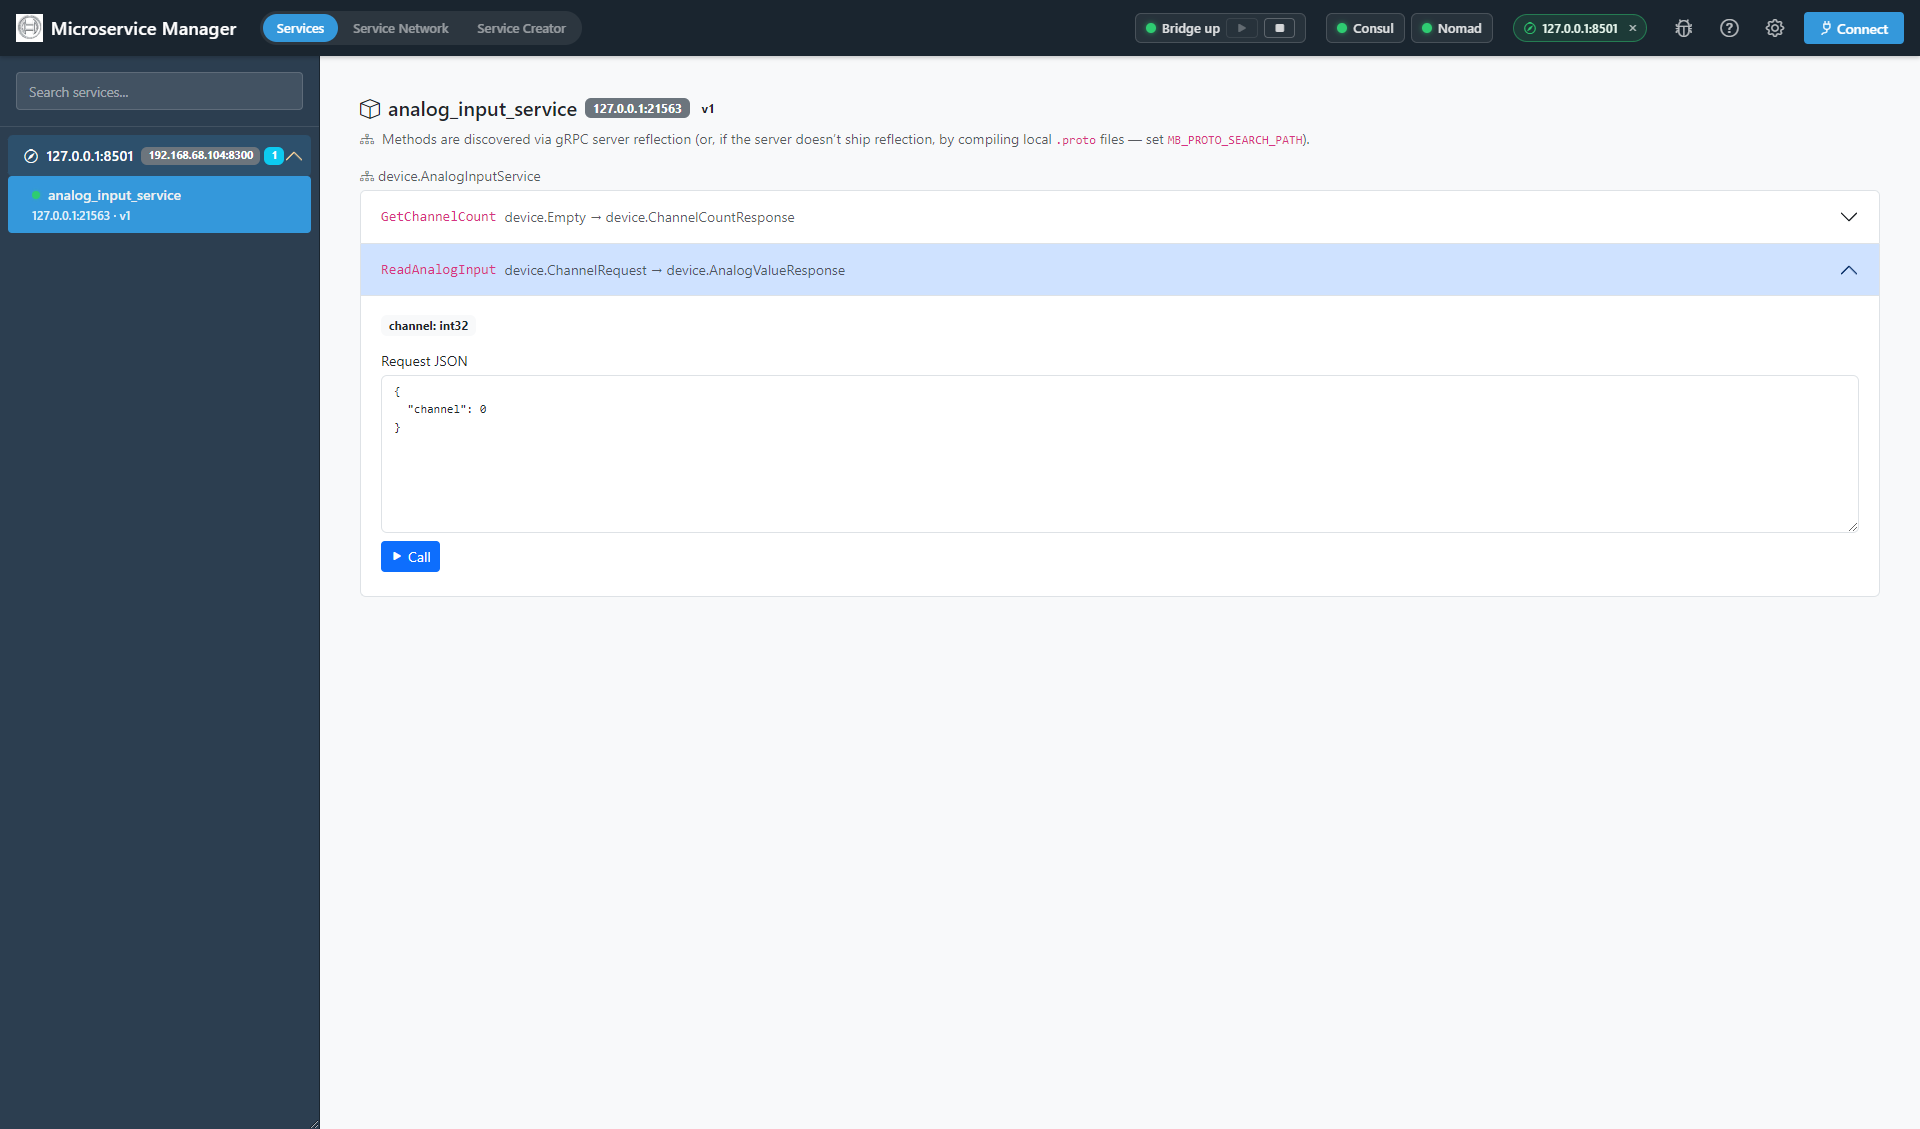
\includegraphics[width=0.95\textwidth]{pictures/Services/api_explorer.png}\\[0.3em]
{\small\textit{Services tab -- API explorer with reflection-driven method list and generic invoke form}}
\end{center}
\vspace{0.5em}

\subsubsection{Service Network Tab}

The \textbf{Service Network} tab has two sub-tabs: \textbf{Nomad} (default) and
\textbf{Consul}.  Both follow the same pattern: a \emph{status} card at the top with
\textbf{Start agent} / \textbf{Stop agent} buttons (configurable address, data dir,
log file), and a \emph{dashboard} below that lists what the agent currently knows
about.

\begin{description}
   \item[Nomad sub-tab] Shows running jobs, allocations, and per-task status.  A
        \textbf{Submit Job} dialog accepts a \texttt{.nomad.hcl} file picker (or
        paste-text), parses it locally, and POSTs to \texttt{/v1/jobs}.  Job logs
        stream into a side panel via the Nomad agent's \texttt{logs} endpoint.
   \item[Consul sub-tab] Shows the service catalog as Consul sees it -- service names,
        IDs, host:port pairs, tags, health-check status, and the
        \texttt{grpc\_services} meta.  Useful for confirming a freshly-deployed
        service really did register (and that its health check is passing).
\end{description}

\vspace{0.5em}
\begin{center}
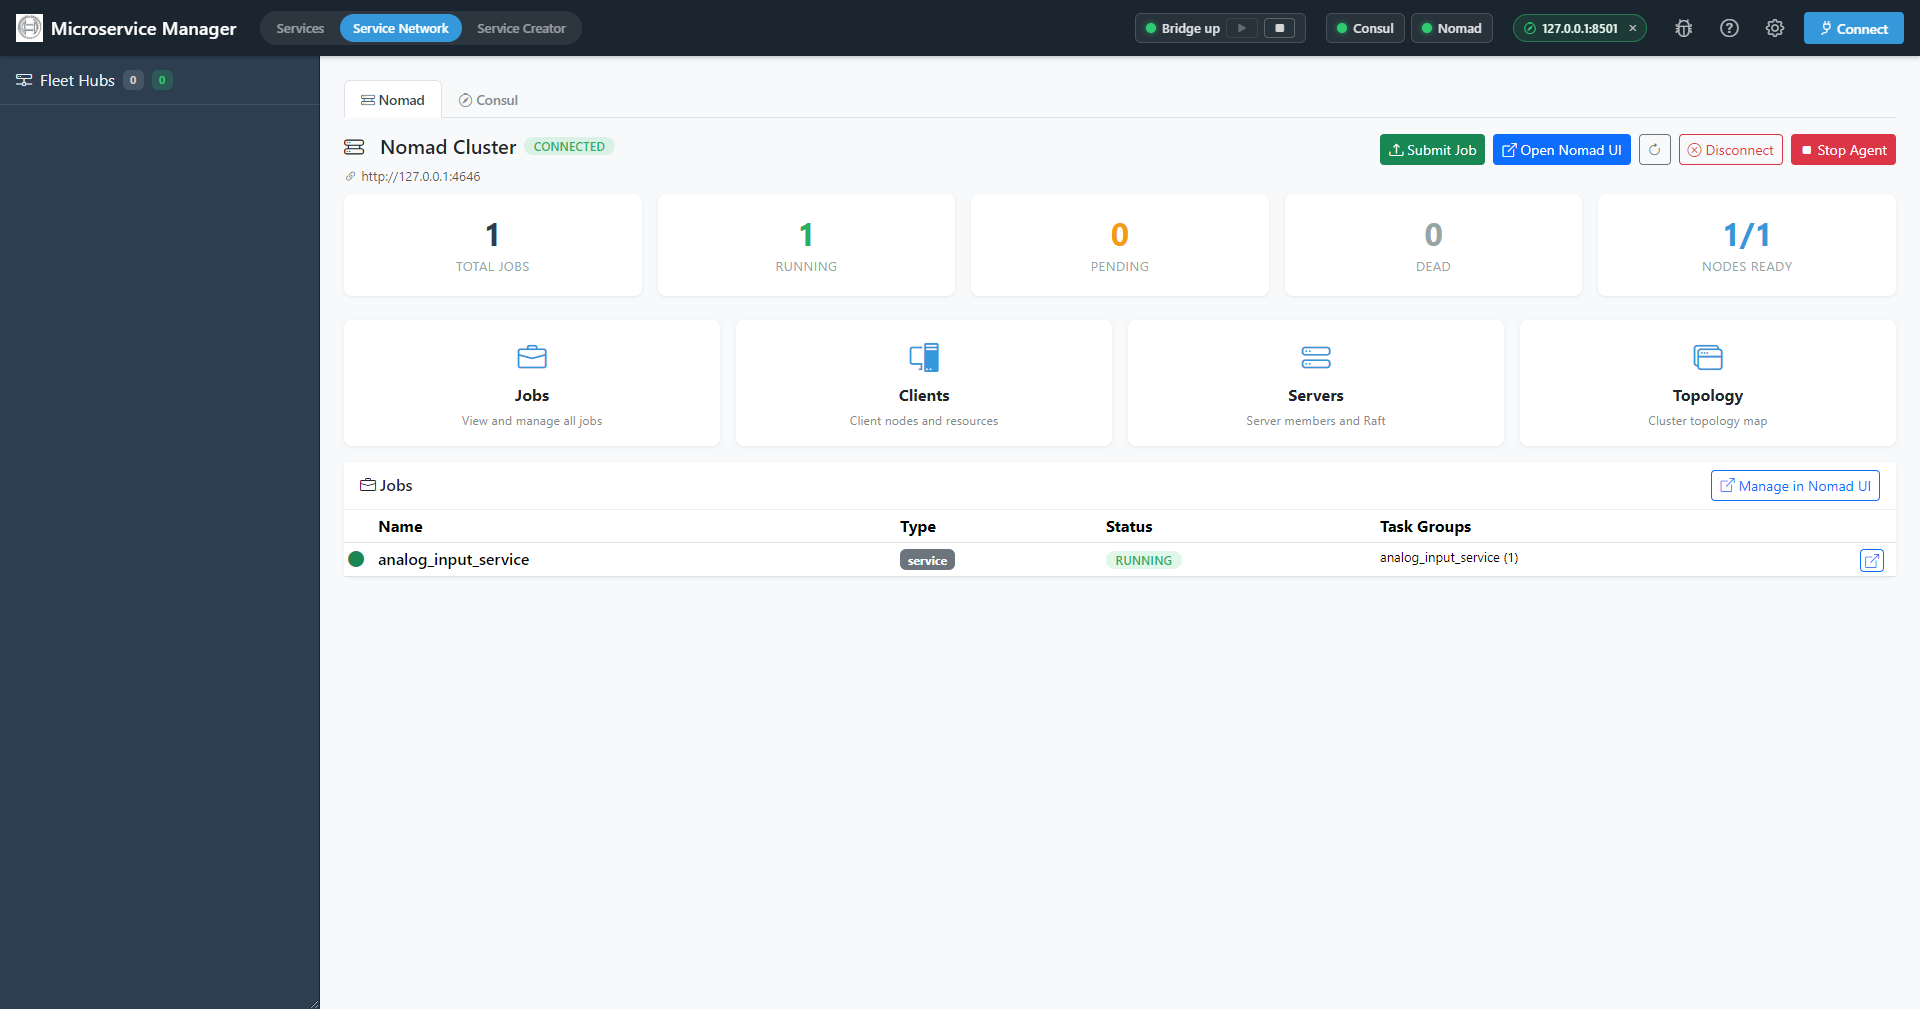
\includegraphics[width=0.95\textwidth]{pictures/ServiceNetwork/Nomad/nomad_dashboard.png}\\[0.3em]
{\small\textit{Service Network -- Nomad dashboard with jobs, allocations, and per-task status}}
\end{center}
\vspace{0.5em}

\vspace{0.5em}
\begin{center}
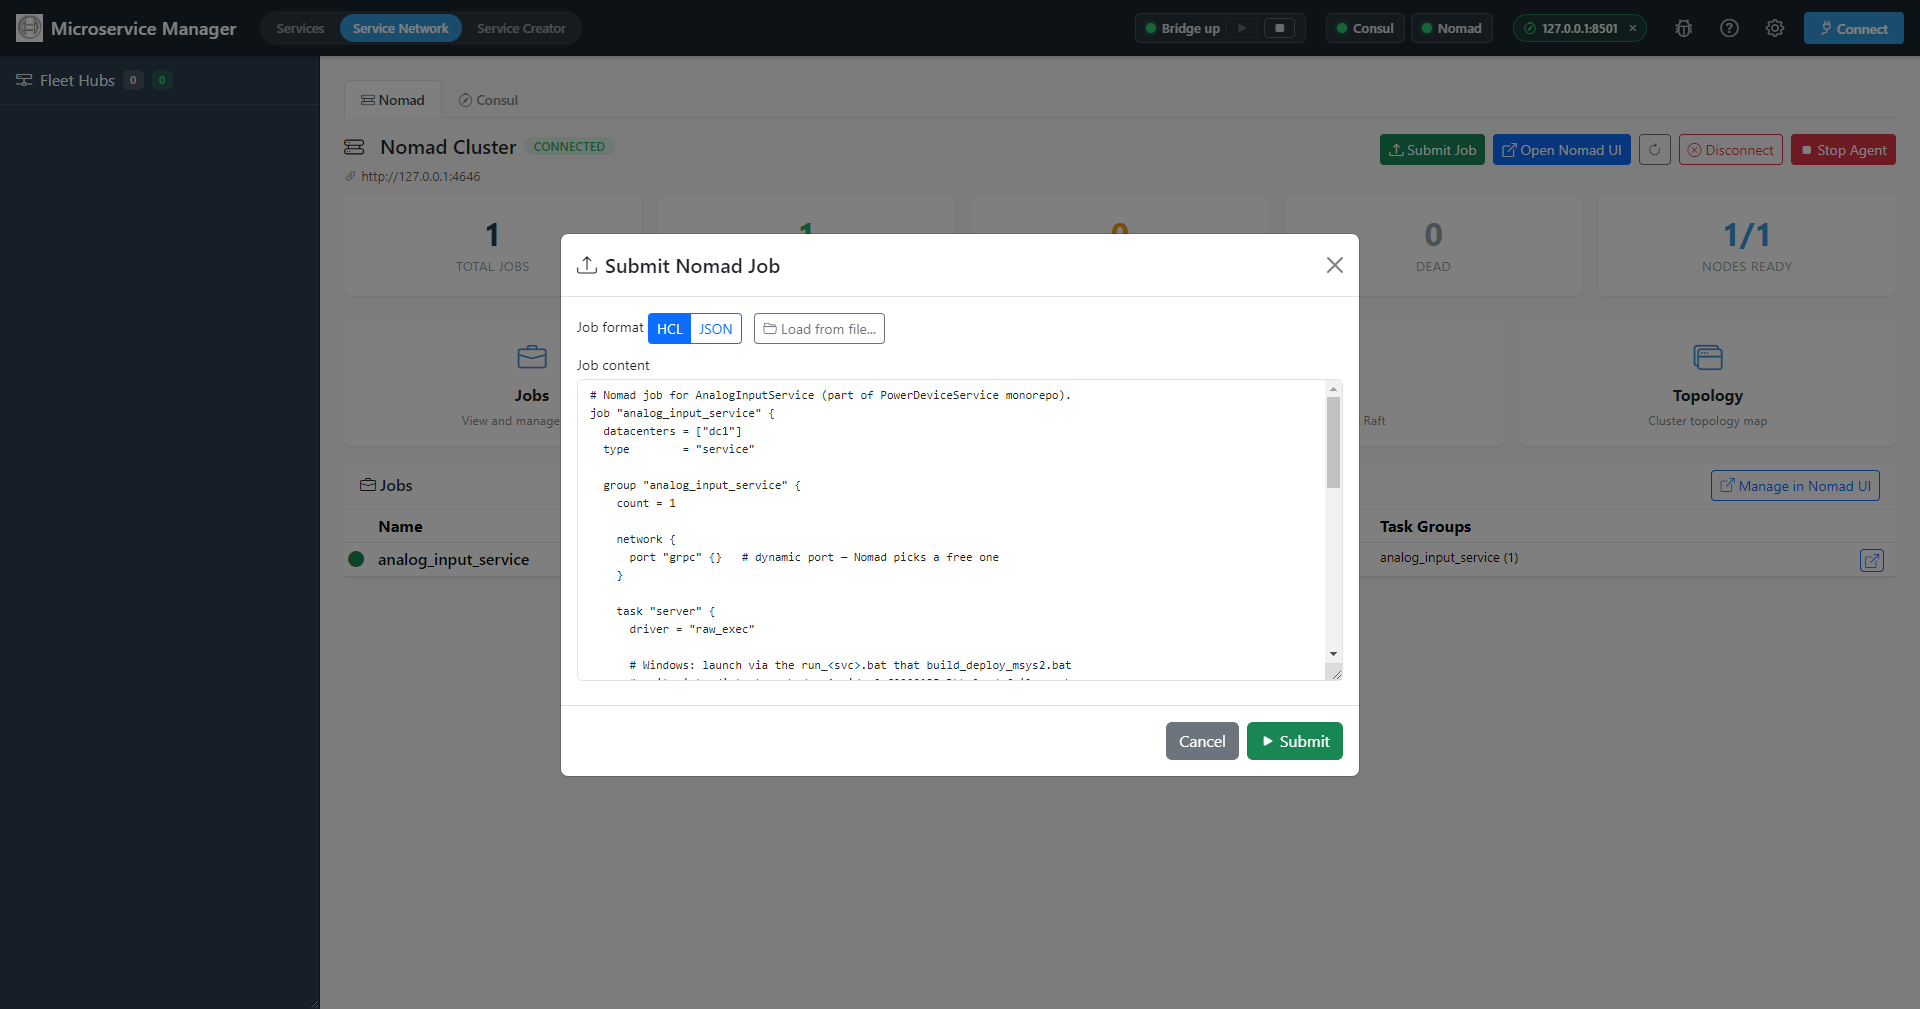
\includegraphics[width=0.85\textwidth]{pictures/ServiceNetwork/Nomad/nomad_submit_job.png}\\[0.3em]
{\small\textit{Submit Job dialog -- file picker for \texttt{.nomad.hcl}}}
\end{center}
\vspace{0.5em}

\vspace{0.5em}
\begin{center}
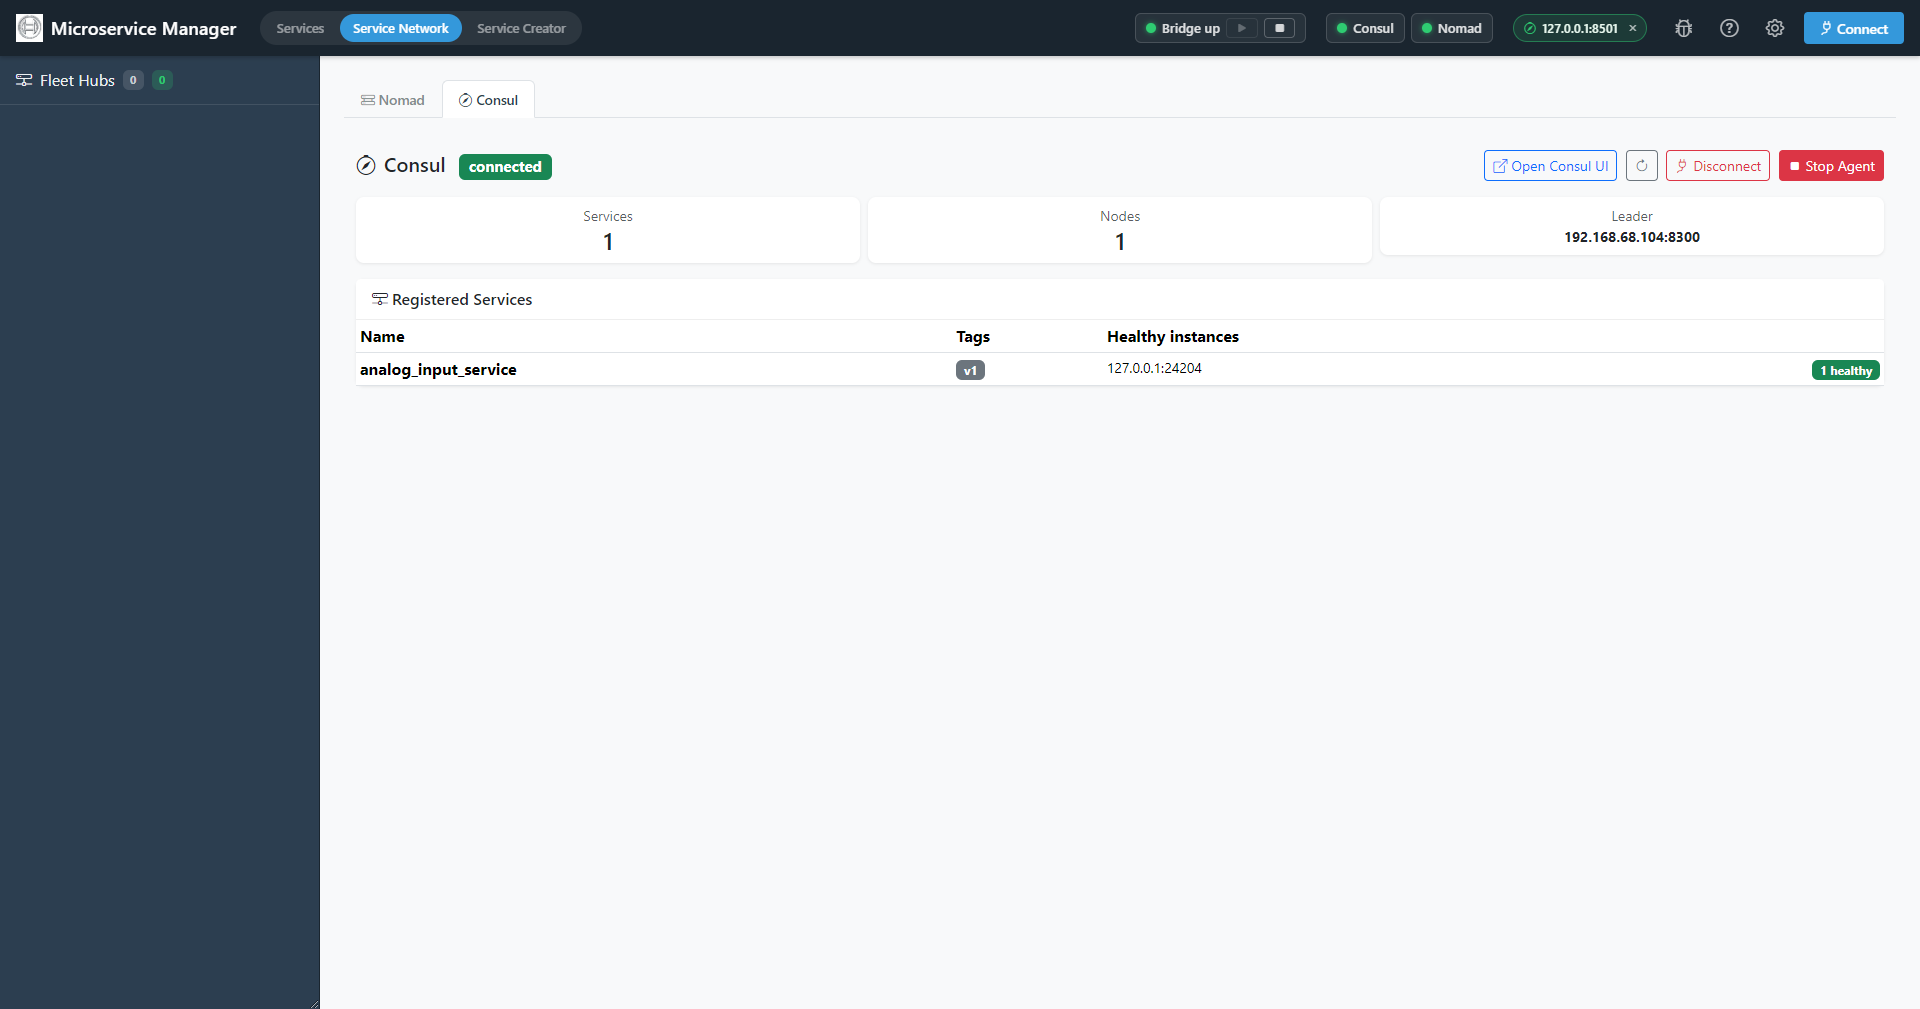
\includegraphics[width=0.95\textwidth]{pictures/ServiceNetwork/Consul/consul_dashboard.png}\\[0.3em]
{\small\textit{Service Network -- Consul service catalog with health-check status}}
\end{center}
\vspace{0.5em}

\subsubsection{Service Creator Wizard}

The \textbf{Service Creator} tab is a four-step wizard for generating a new service
project.  Behind the scenes it POSTs to \texttt{/api/scaffold/generate-v2}; the same
specification can be given to \texttt{mb-scaffold} on the command line.

\paragraph{Step 1: Basic Information}

\vspace{0.5em}
\begin{center}
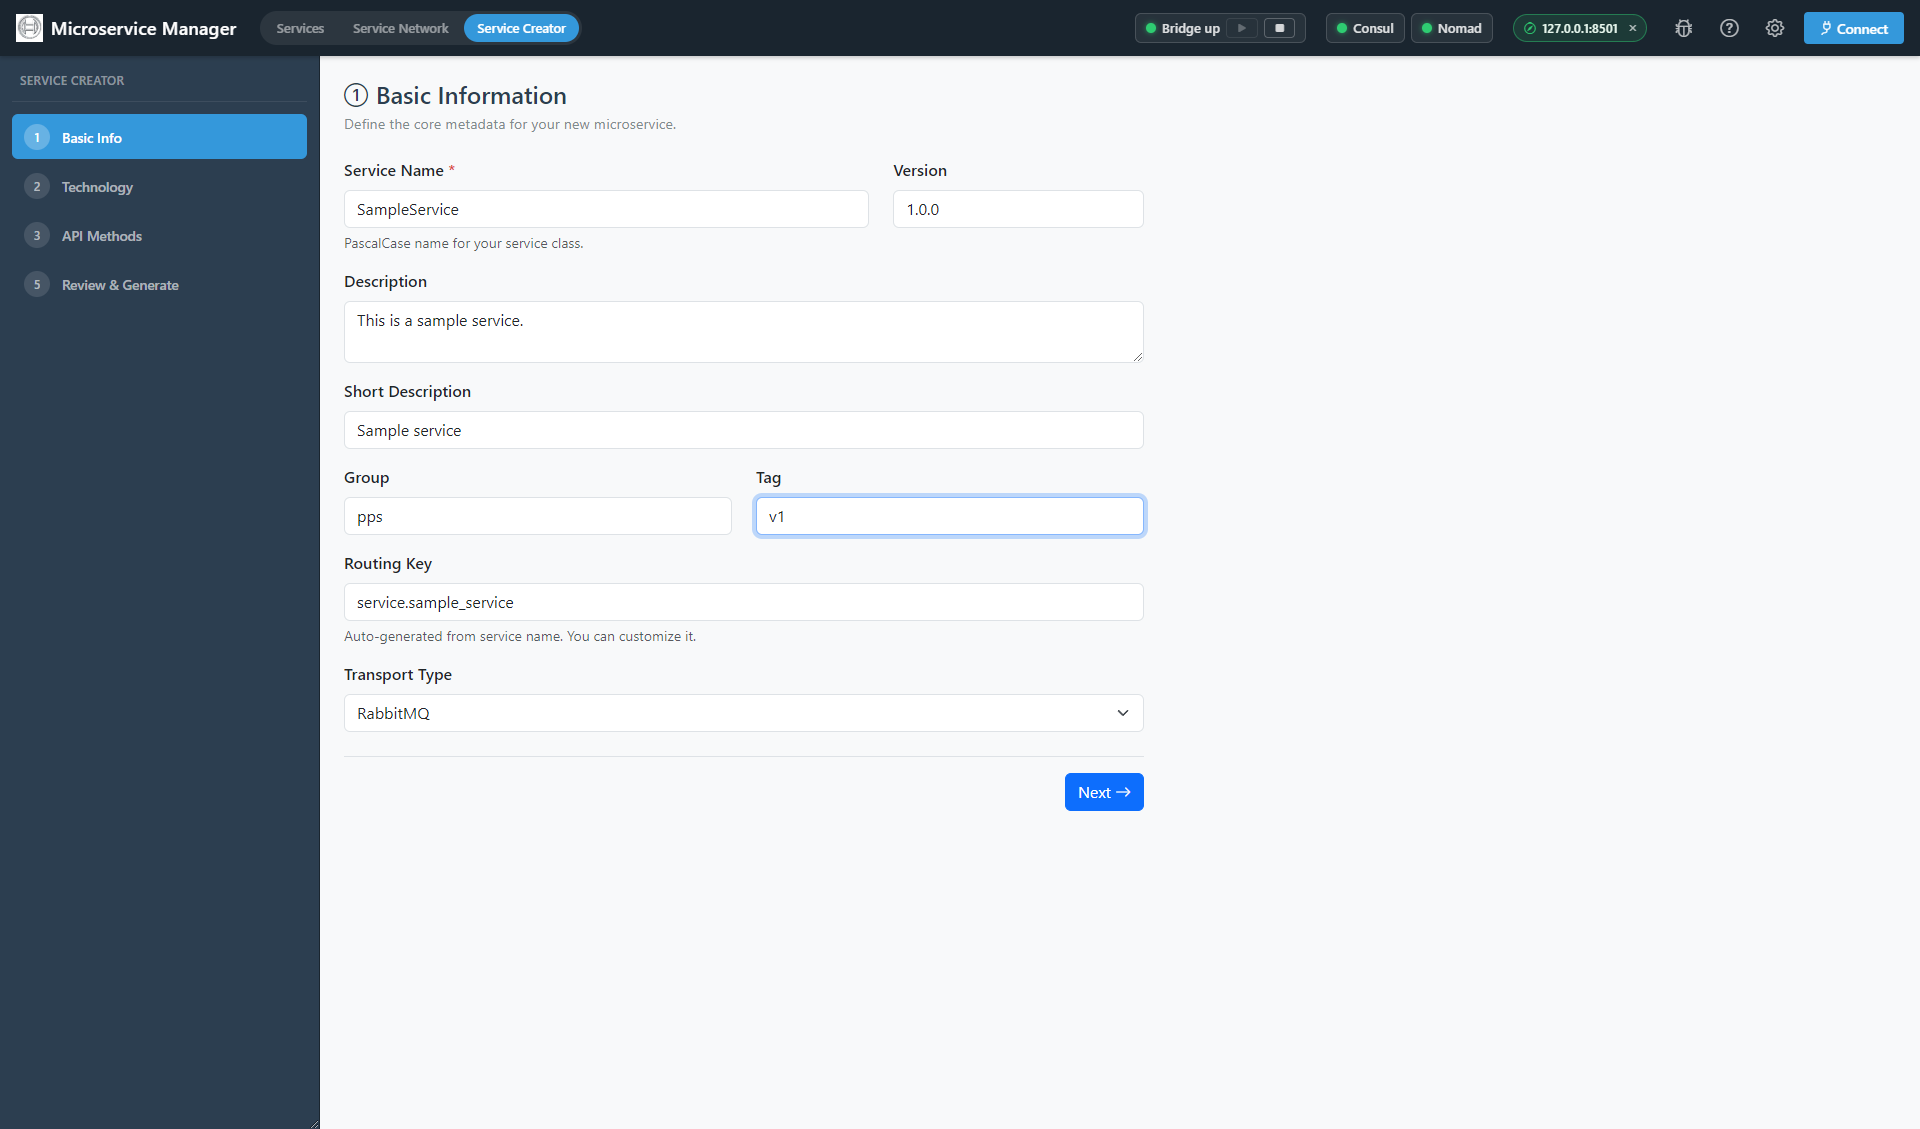
\includegraphics[width=0.85\textwidth]{pictures/ServiceCreator/01_Basic_Info.png}\\[0.3em]
{\small\textit{Service Creator -- Step 1: Basic Information}}
\end{center}
\vspace{0.5em}

\noindent
Define the core metadata for the new service: \textbf{Service Name} (PascalCase),
\textbf{Version}, \textbf{Description / Short description}, \textbf{Group} (for
sidebar organisation in the GUI), \textbf{Tag}, and \textbf{Language} (Python or C++).
The \textbf{Layout} selector picks between \texttt{monorepo}, \texttt{multi\_proto},
and \texttt{separate}.  In \texttt{multi\_proto} mode the wizard also lets you import
multiple existing \texttt{.proto} files in one shot.

\paragraph{Step 2: API Methods}

\vspace{0.5em}
\begin{center}
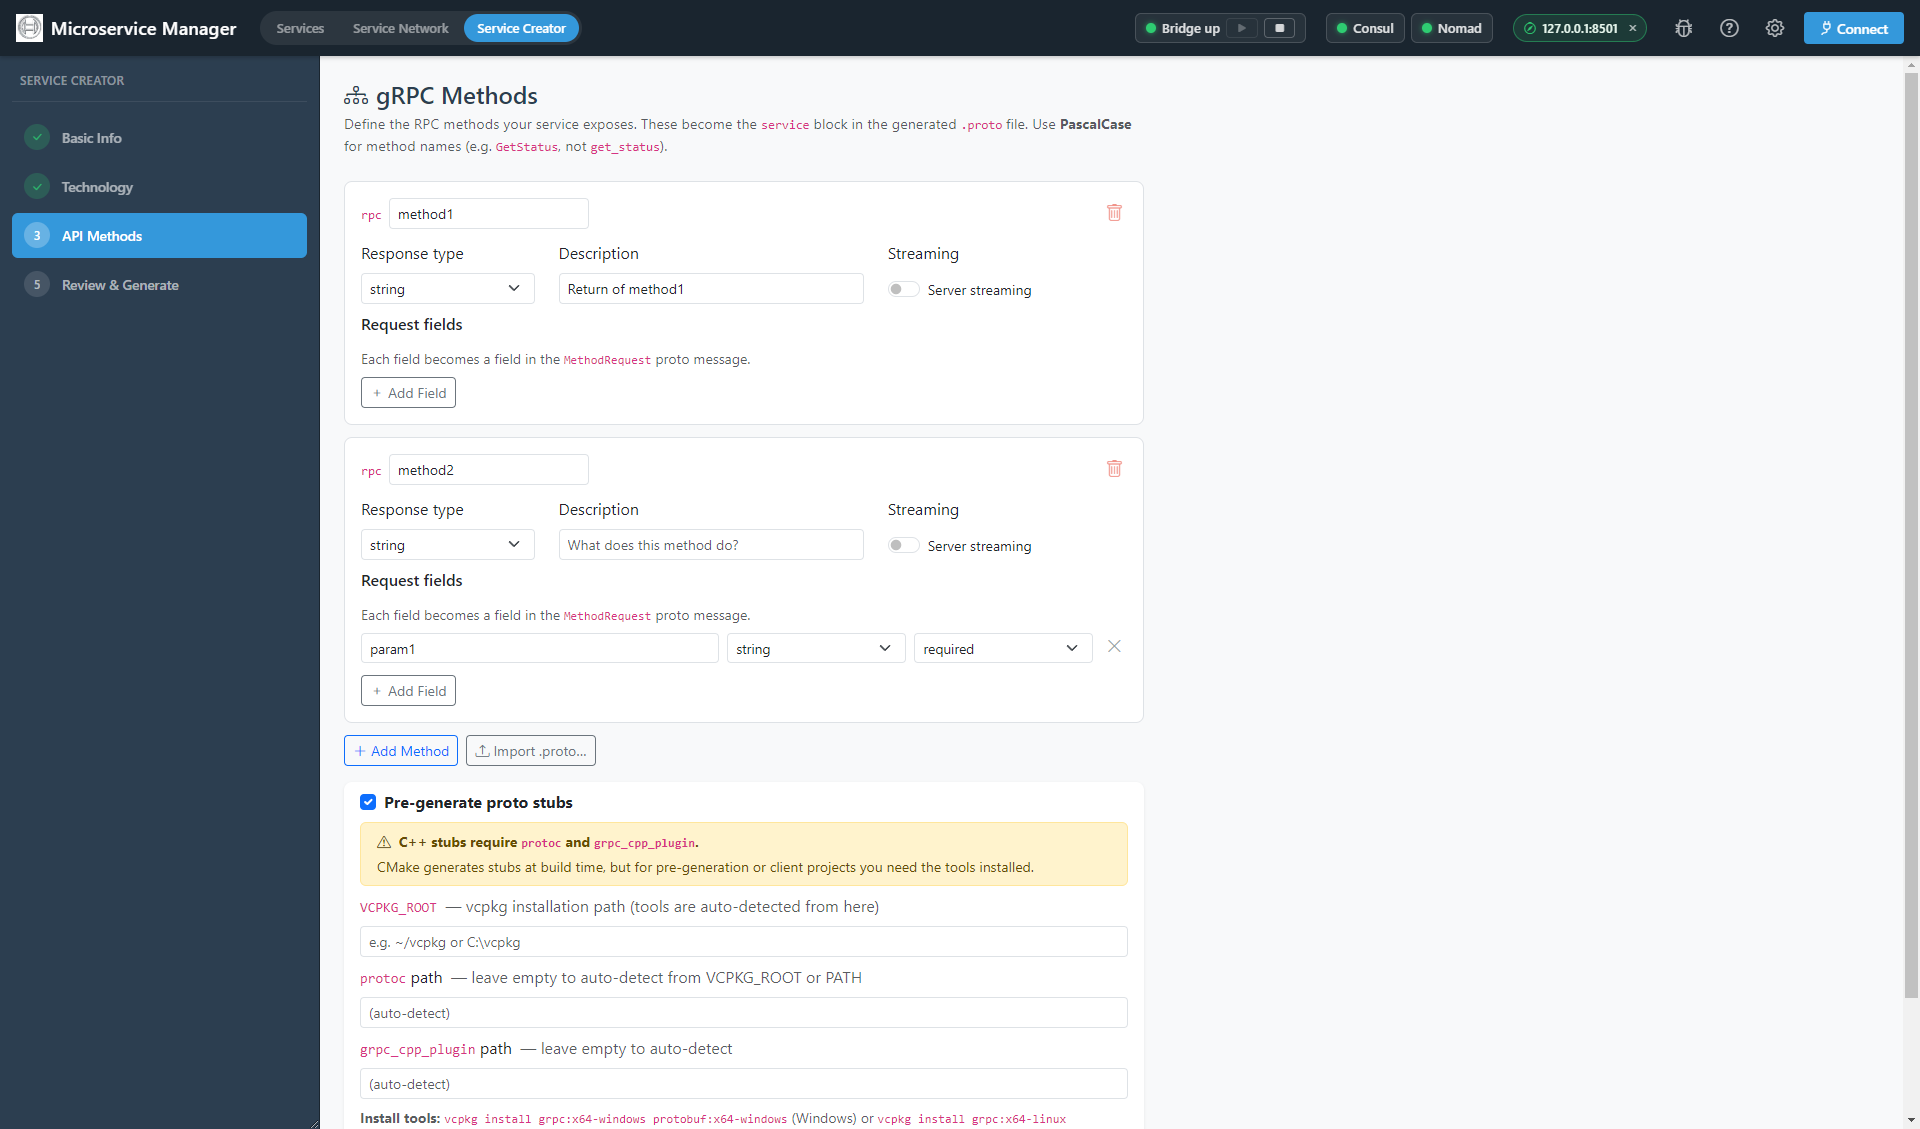
\includegraphics[width=0.85\textwidth]{pictures/ServiceCreator/02_API_Methods.png}\\[0.3em]
{\small\textit{Service Creator -- Step 2: API Methods}}
\end{center}
\vspace{0.5em}

\noindent
Define the methods the service will expose.  Each method has a name (becomes a gRPC
RPC), a return type, a description (becomes the docstring / Doxygen block), and a list
of parameters with name + type + condition (\texttt{required} / \texttt{optional}).
The wizard renders the equivalent \texttt{.proto} text live in a side panel.

\paragraph{Step 3: GUI Support}

\vspace{0.5em}
\begin{center}
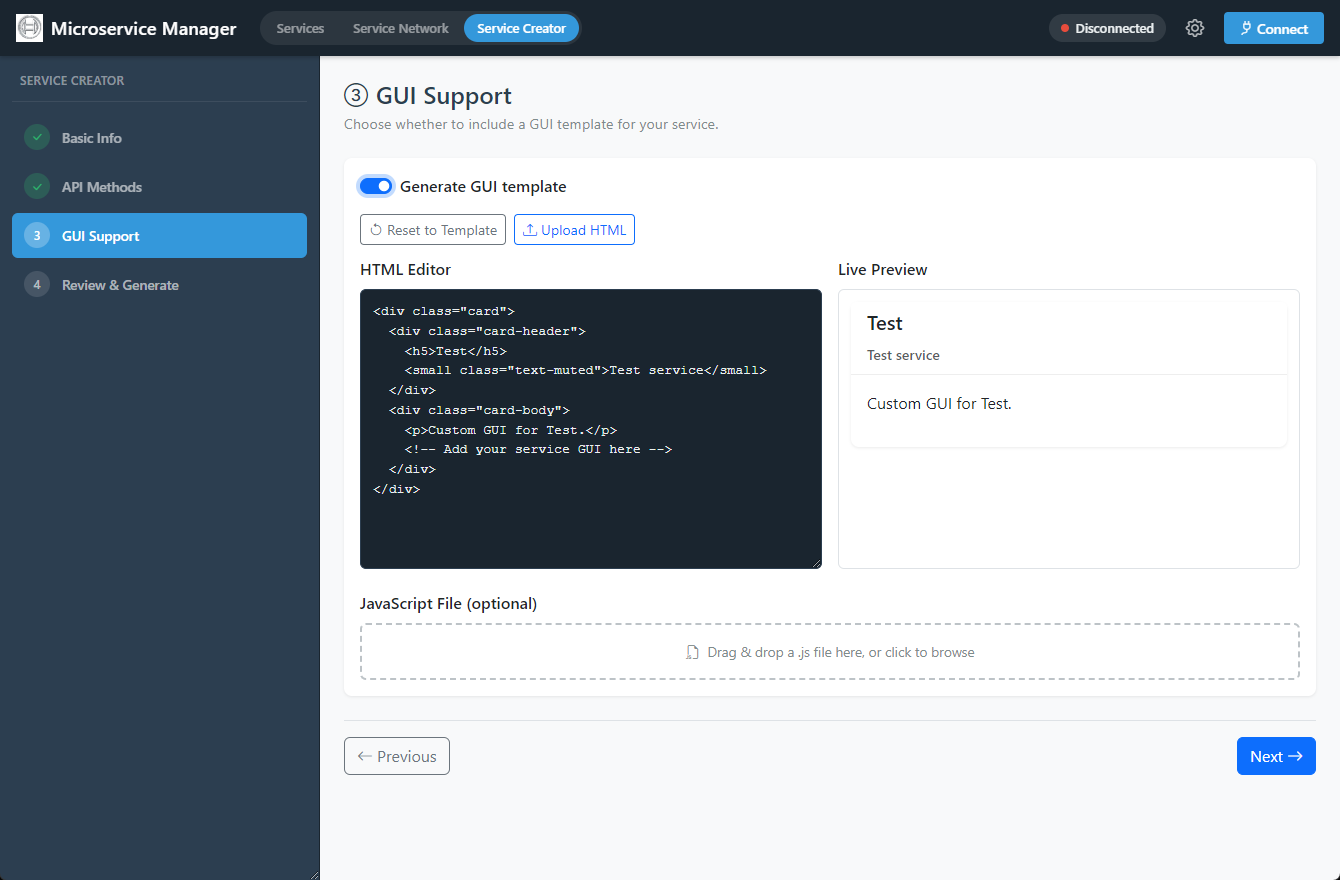
\includegraphics[width=0.85\textwidth]{pictures/ServiceCreator/03_GUI_support.png}\\[0.3em]
{\small\textit{Service Creator -- Step 3: GUI Support}}
\end{center}
\vspace{0.5em}

\noindent
Choose whether to include a custom GUI plugin.  When the \emph{Generate GUI template}
toggle is on, the wizard offers two complementary editors that you can mix and match:

\begin{itemize}
   \item \textbf{Schema Builder} -- a visual form designer that emits a Bootstrap card
         + JS pair driven by a JSON schema (best for parameter-form services)
   \item \textbf{Custom HTML / JS editor} -- a Monaco-style live editor with a
         \emph{Live preview} panel (best for non-form layouts; full access to
         \texttt{window.MicroserviceManager} / \texttt{MM})
\end{itemize}

\paragraph{Step 4: Review and Generate}

\vspace{0.5em}
\begin{center}
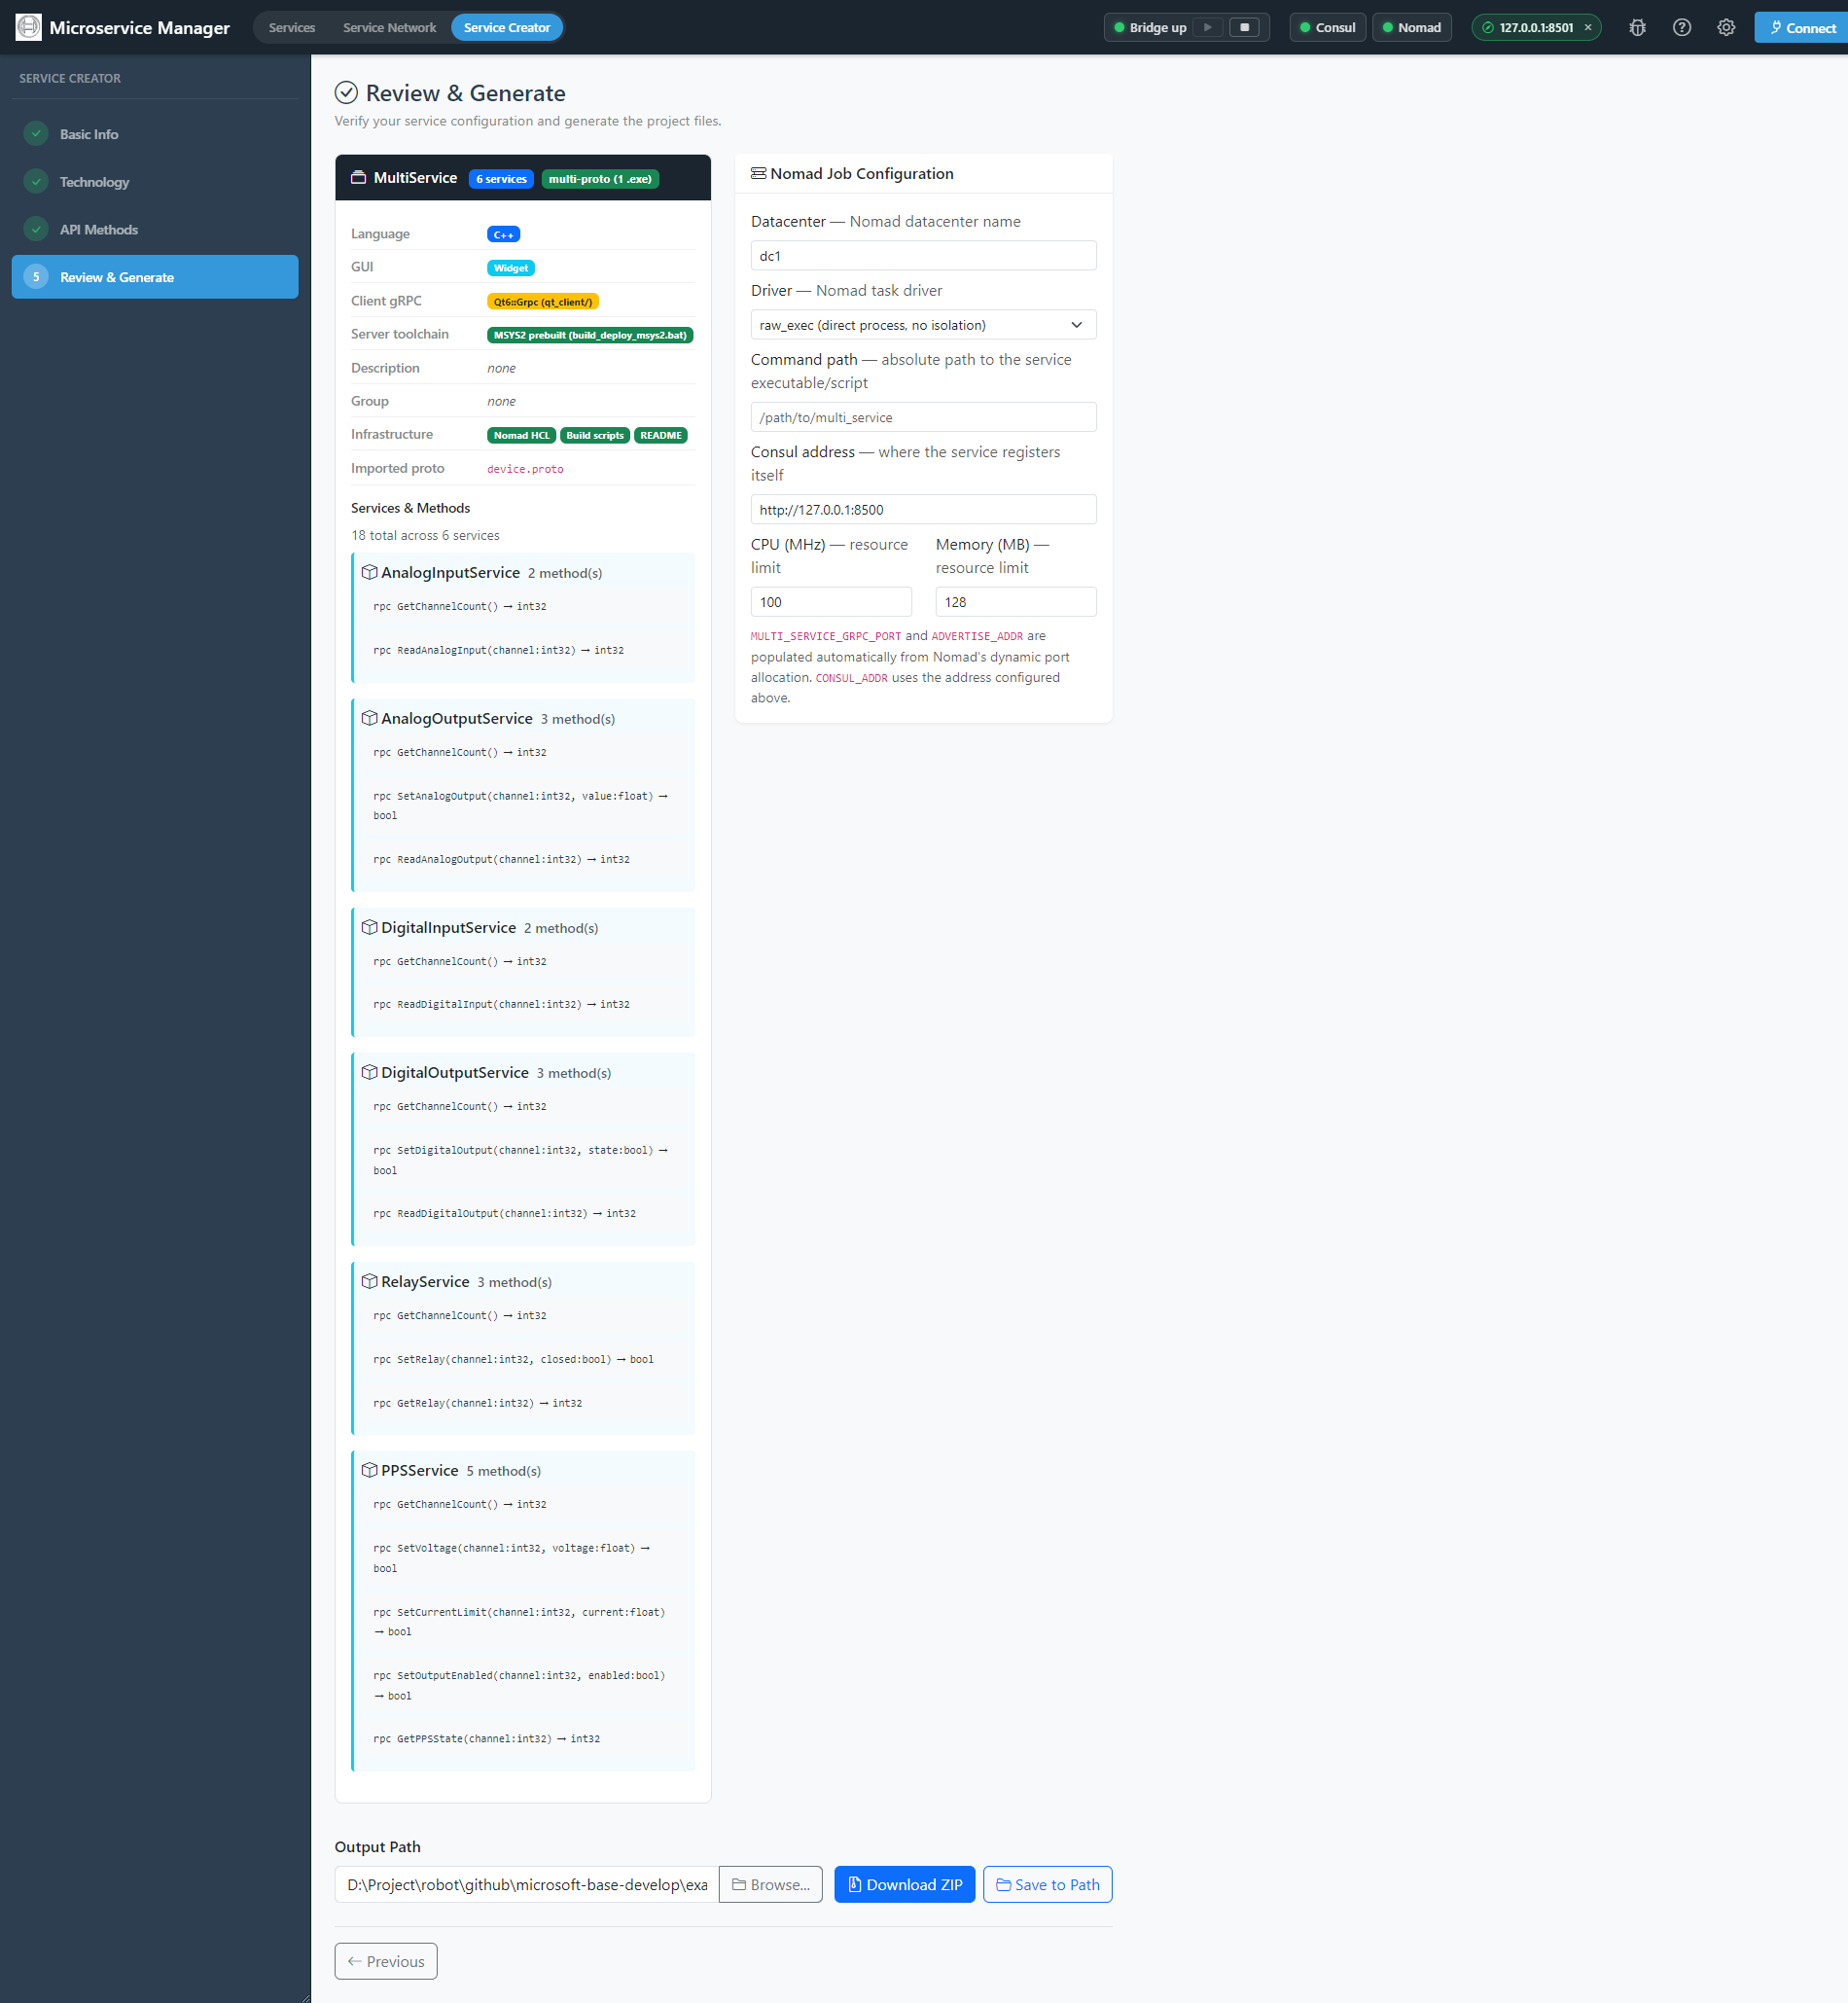
\includegraphics[width=0.85\textwidth]{pictures/ServiceCreator/04_Review_Gen.png}\\[0.3em]
{\small\textit{Service Creator -- Step 4: Review and Generate}}
\end{center}
\vspace{0.5em}

\noindent
The summary card shows every choice you made -- name, layout, language, methods, GUI
toggle.  The \textbf{Generated File Structure} preview lists every file the wizard is
about to write, with the same generic / specific colouring used elsewhere in the docs.
Specify an \textbf{Output Path} to save directly to disk, or leave it blank to
\textbf{Download ZIP}.  Once generated, the project can be built and submitted to
Nomad with the commands printed in the project's own \texttt{README.md}.

% ============================================================================
\subsection{Nomad Job Configuration}
% ============================================================================

Each generated service gets a \texttt{deploy/<svc>.nomad.hcl} job -- a short HCL file
that Nomad runs verbatim.  A typical multi-port service looks like:

\begin{verbatim}
job "calculator_service" {
  datacenters = ["dc1"]
  type        = "service"

  group "calc" {
    count = 1

    network {
      port "grpc" {}                # dynamic port
    }

    service {
      name = "calculator_service"
      port = "grpc"
      tags = ["v1"]
      meta {
        grpc_services = "calc.Calculator"
      }
      check {
        type     = "tcp"
        port     = "grpc"
        interval = "5s"
        timeout  = "1s"
      }
    }

    task "calc" {
      driver = "raw_exec"
      config {
        command = "${NOMAD_TASK_DIR}/calculator_service.exe"
        args    = []
      }
      env {
        CONSUL_ADDR = "http://127.0.0.1:8500"
        GRPC_PORT   = "${NOMAD_PORT_grpc}"
      }
      resources { cpu = 100 memory = 128 }
    }
  }
}
\end{verbatim}

\noindent
The Service Creator wizard generates this file for every service automatically.
For multi-proto layouts, a single job hosts all the services on one port and
registers each one separately under its own Consul name.

% ============================================================================
\subsection{Process Lifecycle}
% ============================================================================

The lifecycle of a service process is the same on Windows and Linux:

\begin{figure}[!htb]
\centering

\includegraphics[width=0.7\textwidth]{pictures/state_process_lifecycle.png}
\caption{Service Process Lifecycle States}
\label{fig:state_process_lifecycle}
\end{figure}

\begin{enumerate}
   \item \textbf{Spawn} -- Nomad's \texttt{raw\_exec} driver launches the binary with
         a dynamic \texttt{NOMAD\_PORT\_grpc} and the \texttt{CONSUL\_ADDR} env var
   \item \textbf{Bind \& Register} -- the service binds the gRPC server, then calls
         \texttt{register\_service()} against the local Consul agent
   \item \textbf{Serve} -- Consul's TCP health check polls the gRPC port; the bridge
         resolves the service via Consul and routes calls
   \item \textbf{Shutdown} -- on \texttt{SIGBREAK} (Windows) or \texttt{SIGTERM}
         (Linux), the service deregisters from Consul and lets the gRPC server
         drain.  Critical Windows fix: the default \texttt{SIGBREAK} handler calls
         \texttt{ExitProcess} (no Python \texttt{KeyboardInterrupt}, no
         \texttt{finally} blocks) -- the framework explicitly installs
         \texttt{signal.default\_int\_handler} so SIGBREAK becomes
         \texttt{KeyboardInterrupt} and the deregister-then-exit path runs cleanly
\end{enumerate}

% ============================================================================
\subsection{Installation}
% ============================================================================

\subsubsection{From Source}

\begin{verbatim}
git clone https://github.com/test-fullautomation/python-microservice-base.git
cd python-microservice-base
pip install .

# Development mode
pip install -e .
\end{verbatim}

\noindent
The Consul and Nomad agent binaries must be installed separately.  On Windows:
\texttt{winget install Hashicorp.Consul Hashicorp.Nomad}.  On Debian / Ubuntu:
follow the official \texttt{apt} repo instructions at \href{https://developer.hashicorp.com/well-architected-framework/install}{HashiCorp's
docs}.  The \texttt{bootstrap.sh} script in the Linux installer does this
non-interactively for you.

\subsubsection{Standalone Desktop Installer (DevAtServGUI)}

\begin{itemize}
   \item Run \texttt{build.bat} (Windows, NSIS) or \texttt{build.sh} (Linux) inside
         \texttt{MicroserviceBase/MicroserviceManagerGUI/}
   \item The Windows installer detects existing Consul / Nomad and offers
         \texttt{winget install} when missing
   \item The Linux installer ships \texttt{bootstrap.sh} for AppImage users; \texttt{.deb}
         users get a \texttt{postinst} hook that runs it when stdin is a TTY
\end{itemize}

\subsubsection{GUI from Source}

\begin{verbatim}
cd MicroserviceBase/MicroserviceManagerGUI
npm install
npm start            # Electron mode
# or, for browser mode, just start the bridge and open http://localhost:1112
\end{verbatim}

% ============================================================================
\subsection{Quick Start}
% ============================================================================

\subsubsection{Start the Local Agents}

\begin{verbatim}
consul agent -dev                                      # one terminal
nomad agent -dev -bind=0.0.0.0 -network-interface=lo   # another terminal
\end{verbatim}

\noindent
(Or use the Manager GUI's \textbf{Service Network} tab to start both as managed
subprocesses.)

\subsubsection{Start the FastAPI Bridge}

\begin{verbatim}
python -m MicroserviceBase.adapters.ui_bridge.fastapi_bridge \
    --bridge-port 1112 --consul-addr http://127.0.0.1:8500
\end{verbatim}

\noindent
Open \texttt{http://localhost:1112} for the Manager GUI in browser mode.

\subsubsection{Generate and Run a Service}

\begin{verbatim}
# Python single-service:
python -m MicroserviceBase.tools.scaffold_cli \
    --name calculator_service --language python \
    --layout monorepo --out out/calculator_service \
    --method "Add(a:int,b:int)->int" \
    --method "Multiply(a:int,b:int)->int"

cd out/calculator_service
pip install -r requirements.txt
python scripts/generate_protos.py            # builds *_pb2[_grpc].py
nomad job run deploy/calculator_service.nomad.hcl
\end{verbatim}

\noindent
The service registers itself in Consul on startup; the Manager GUI's Services tab
picks it up automatically.

\subsubsection{Call the Service from Robot Framework}

\begin{verbatim}
*** Settings ***
Library    QConnectBase

*** Test Cases ***
Calculator Should Add
    Connect       grpc://calculator_service@http://127.0.0.1:8500
    ${result}=    Send Command    Calculator.Add    {"a": 1, "b": 2}
    Verify        ${result}       {"result": 3}
    Disconnect
\end{verbatim}

\noindent
The \texttt{grpc://} URL form selects the QConnectBase \texttt{GrpcClient}
connection type; the \texttt{<service\_name>@<consul\_addr>} suffix tells it
to resolve via Consul before opening the channel.

% ============================================================================
\subsection{Diagrams Reference}
% ============================================================================

The following PlantUML diagrams ship in the \texttt{docs/diagrams/} folder.  Older
diagrams from the RabbitMQ era are preserved under
\texttt{docs/diagrams/\_archive/} for historical reference; the active set below
reflects the current gRPC + Consul + Nomad architecture:

\begin{description}
   \item[00\_canonical\_architecture.puml] Canonical end-to-end picture: services,
        Consul, Nomad, FastAPI bridge, GUI, Robot Framework client
   \item[component.puml] Component diagram with package dependencies (current layout)
   \item[class\_domain.puml] Class diagram for the domain layer
        (\texttt{ServiceBase}, value types, generated service classes)
   \item[class\_ports.puml] Class diagram for port interfaces (Transport, Registry,
        Process, Serialization, UIBridge)
   \item[class\_adapters.puml] Class diagram for adapter implementations (gRPC,
        Consul, Nomad, FastAPI bridge, scaffold)
   \item[gui\_architecture.puml] GUI dual-host architecture (Electron + browser)
   \item[sequence\_communication.puml] End-to-end RPC: GUI -- bridge -- Consul -- service
   \item[sequence\_rpc.puml] Single-RPC sequence (reflection-driven invocation)
   \item[sequence\_registration.puml] Service registration flow (Consul HTTP)
   \item[sequence\_shutdown.puml] Graceful deregister-then-shutdown sequence
   \item[sequence\_gui\_plugin\_loading.puml] How service plugins are loaded into the
        Manager GUI namespace
   \item[state\_process\_lifecycle.puml] Service process state machine (spawn,
        register, serve, deregister, exit)
   \item[component\_qt\_*.puml / sequence\_qml\_*.puml] Qt-shell template family
        (Widget, QML, WASM) used by the Service Plugin host
\end{description}
